% --------------------------
% ANÁLISIS DEL CONJUNTO DE DATOS DEPURADO
% --------------------------
En esta sección se presenta un análisis detallado del conjunto de datos, que incluye la identificación de patrones y tendencias en las trayectorias individuales. El conjunto de datos contiene puntos de recorrido obtenidos a lo largo de diez días. Por lo que el primer acercamiento del análisis es poder ver la distribución de los puntos de recorrido en cada día registrado por medio un histrograma por día. Para crear estos histogramas se ejecuta el código del Apéndice \ref{cod:identifier_histogram_daily}. A continuación, se muestran estos histogramas.

\begin{figure}[htbp]
    \centering
    \begin{subfigure}[t]{0.48\textwidth-1em}
        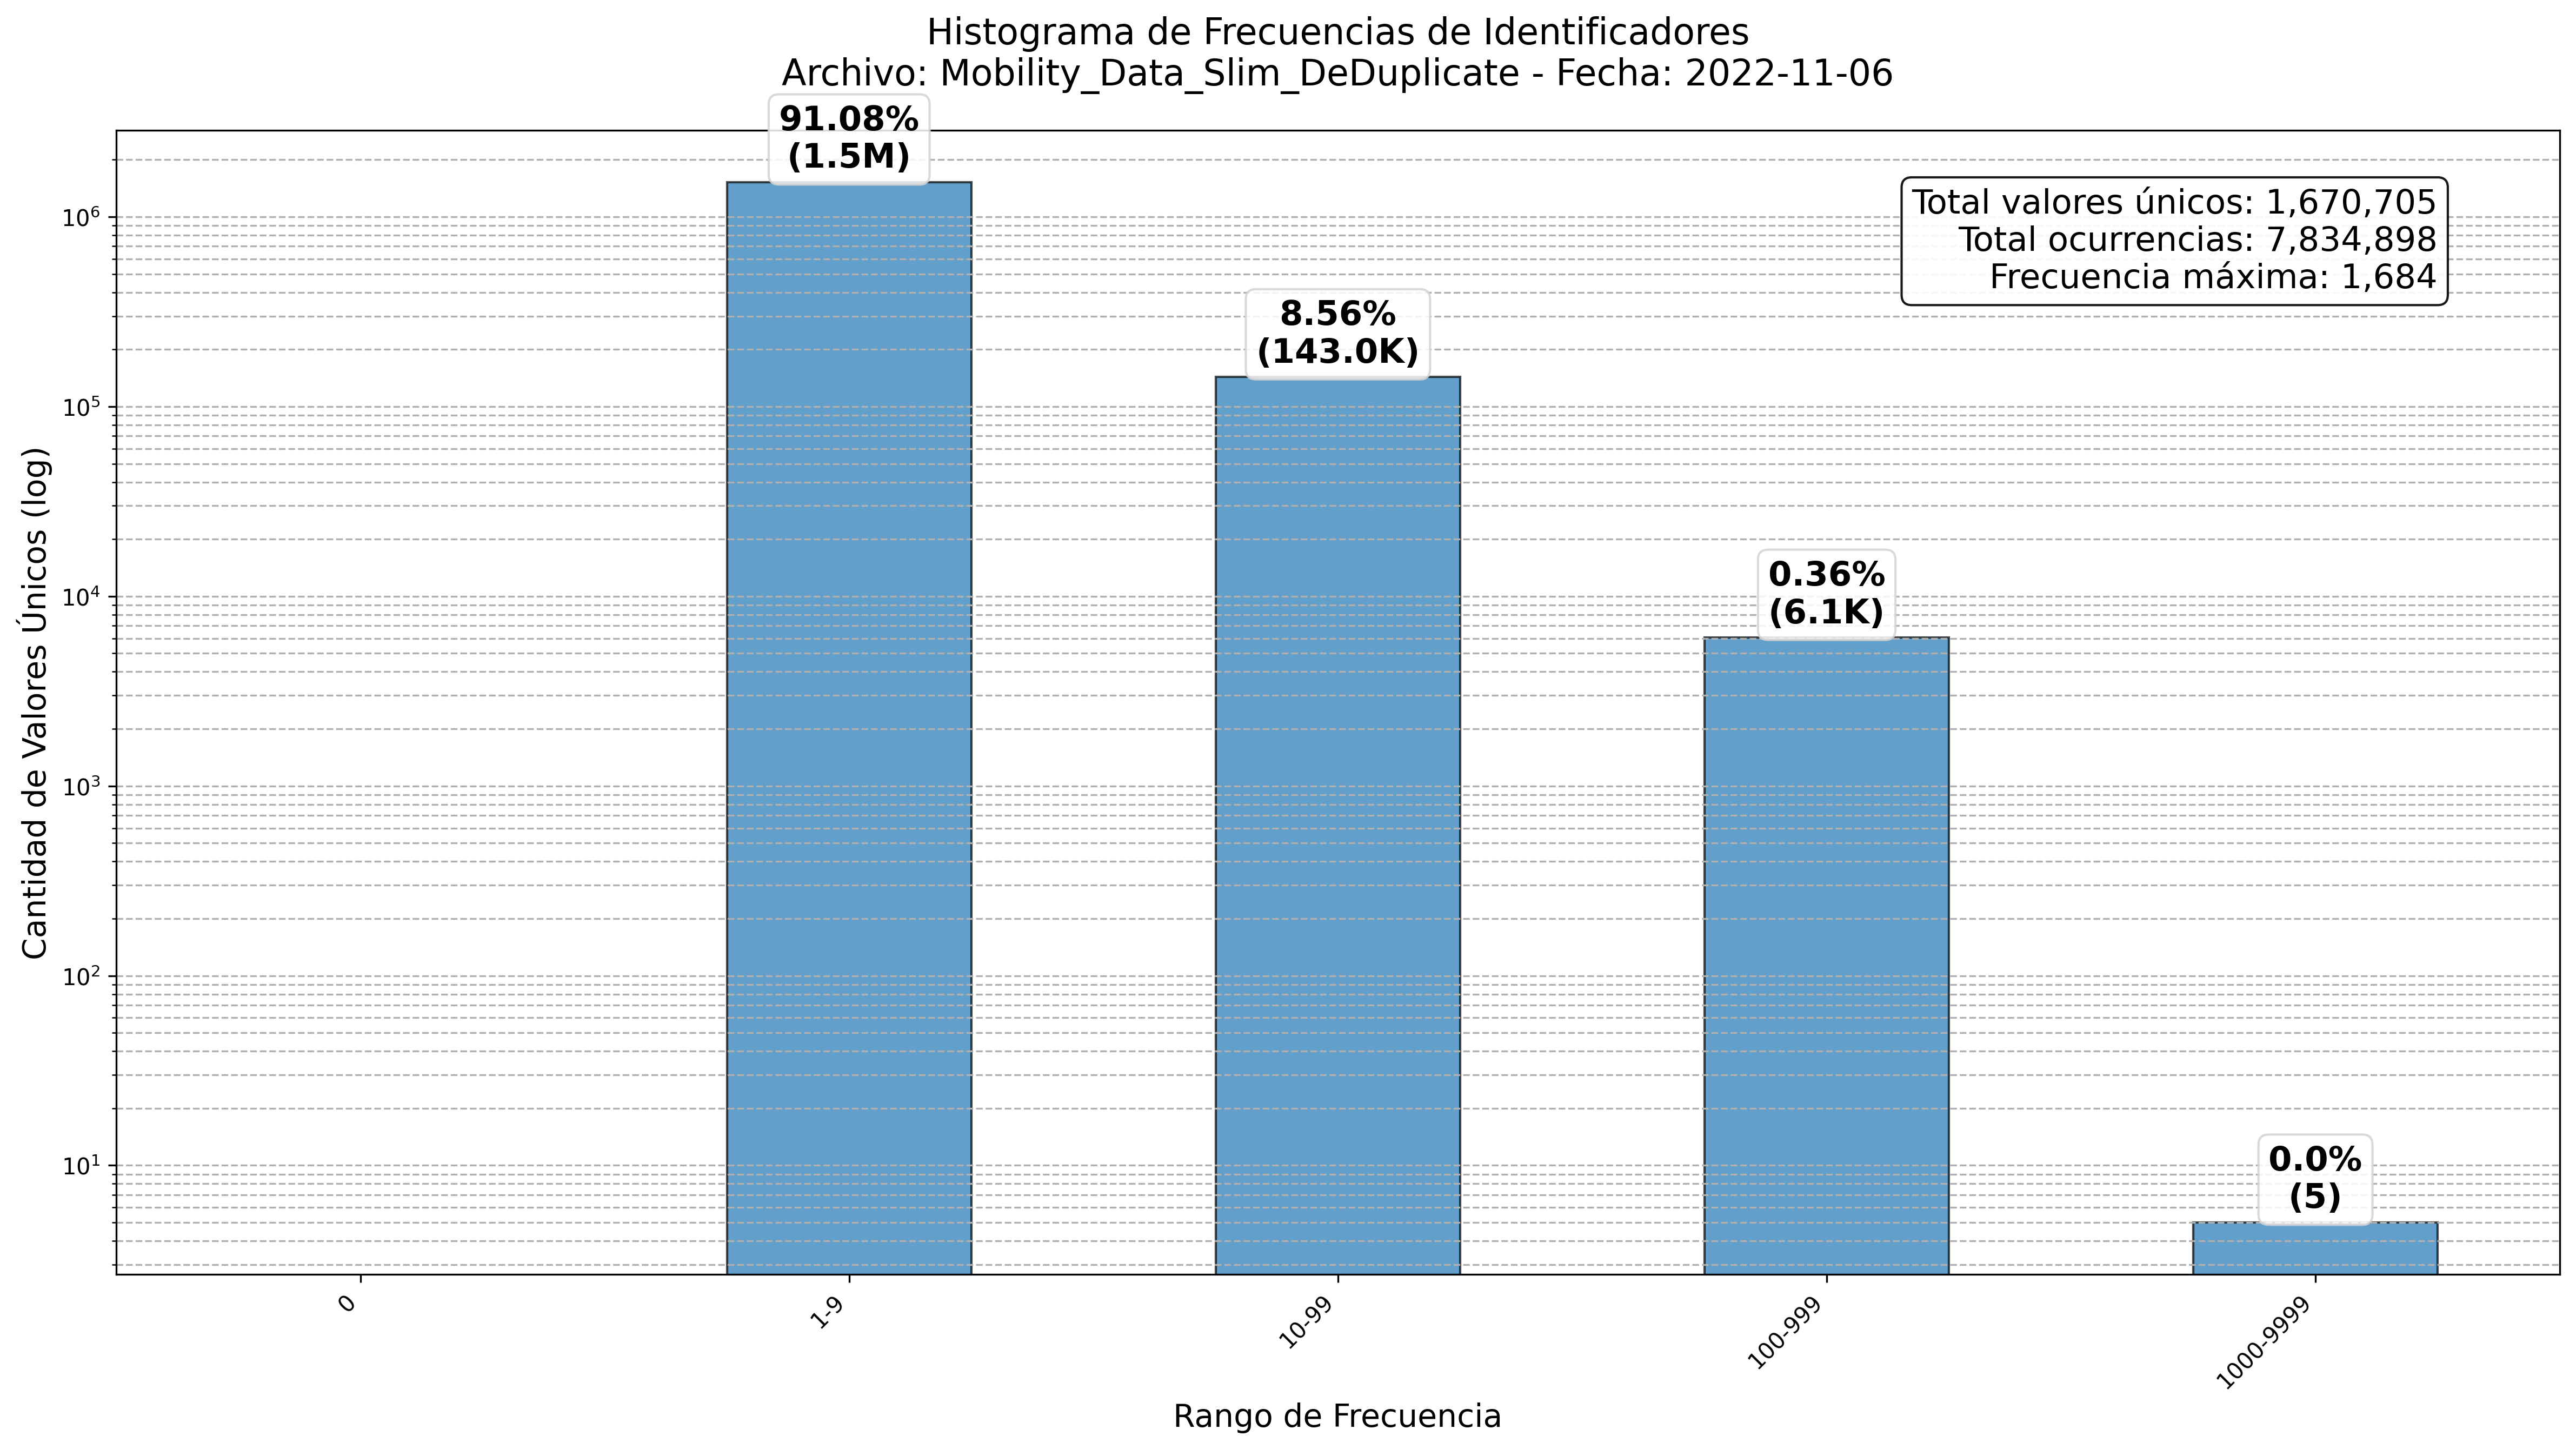
\includegraphics[width=\linewidth]{img/daily_histograms/histograma_identifier_Mobility_Data_Slim_DeDuplicate_2022-11-06.png}
        \caption{Histograma del 06/Nov/2022}
        \label{fig:sub1}
    \end{subfigure}
    \hfill
    \begin{subfigure}[t]{0.48\textwidth-1em}
        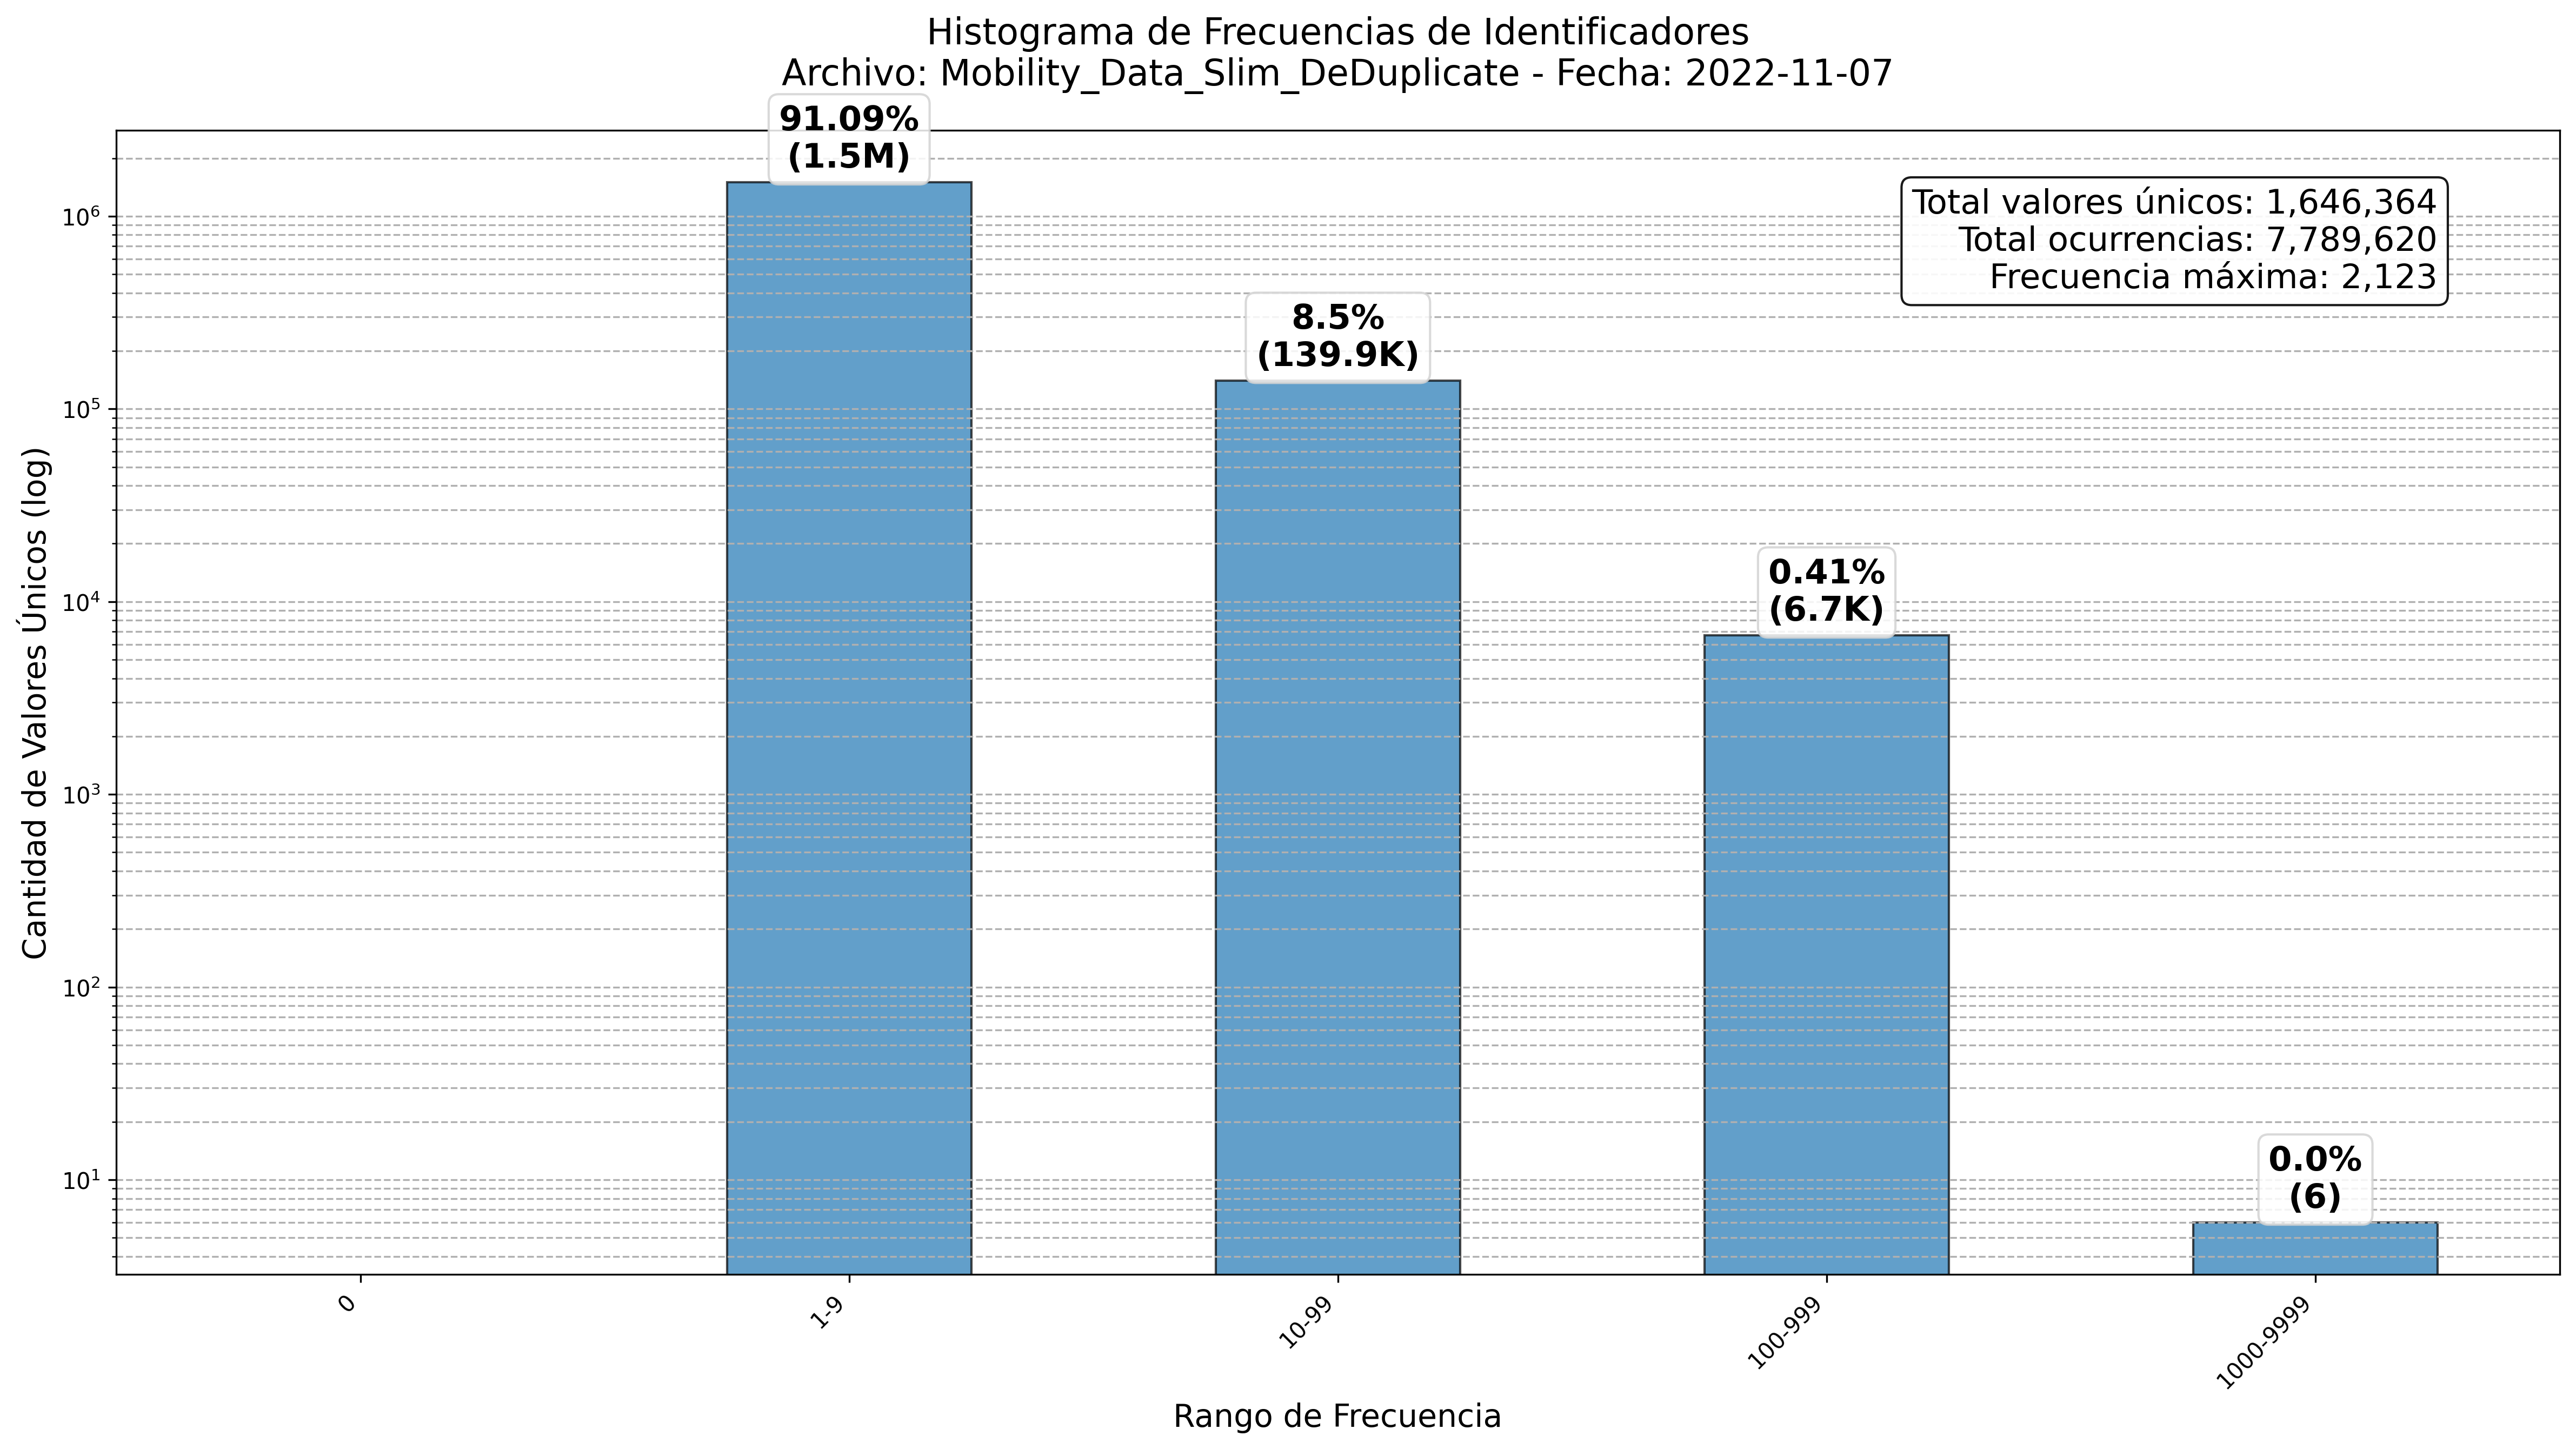
\includegraphics[width=\linewidth]{img/daily_histograms/histograma_identifier_Mobility_Data_Slim_DeDuplicate_2022-11-07.png}
        \caption{Histograma del 07/Nov/2022}
        \label{fig:sub2}
    \end{subfigure}

    \vspace{0.5cm}

    \begin{subfigure}[t]{0.48\textwidth-1em}
        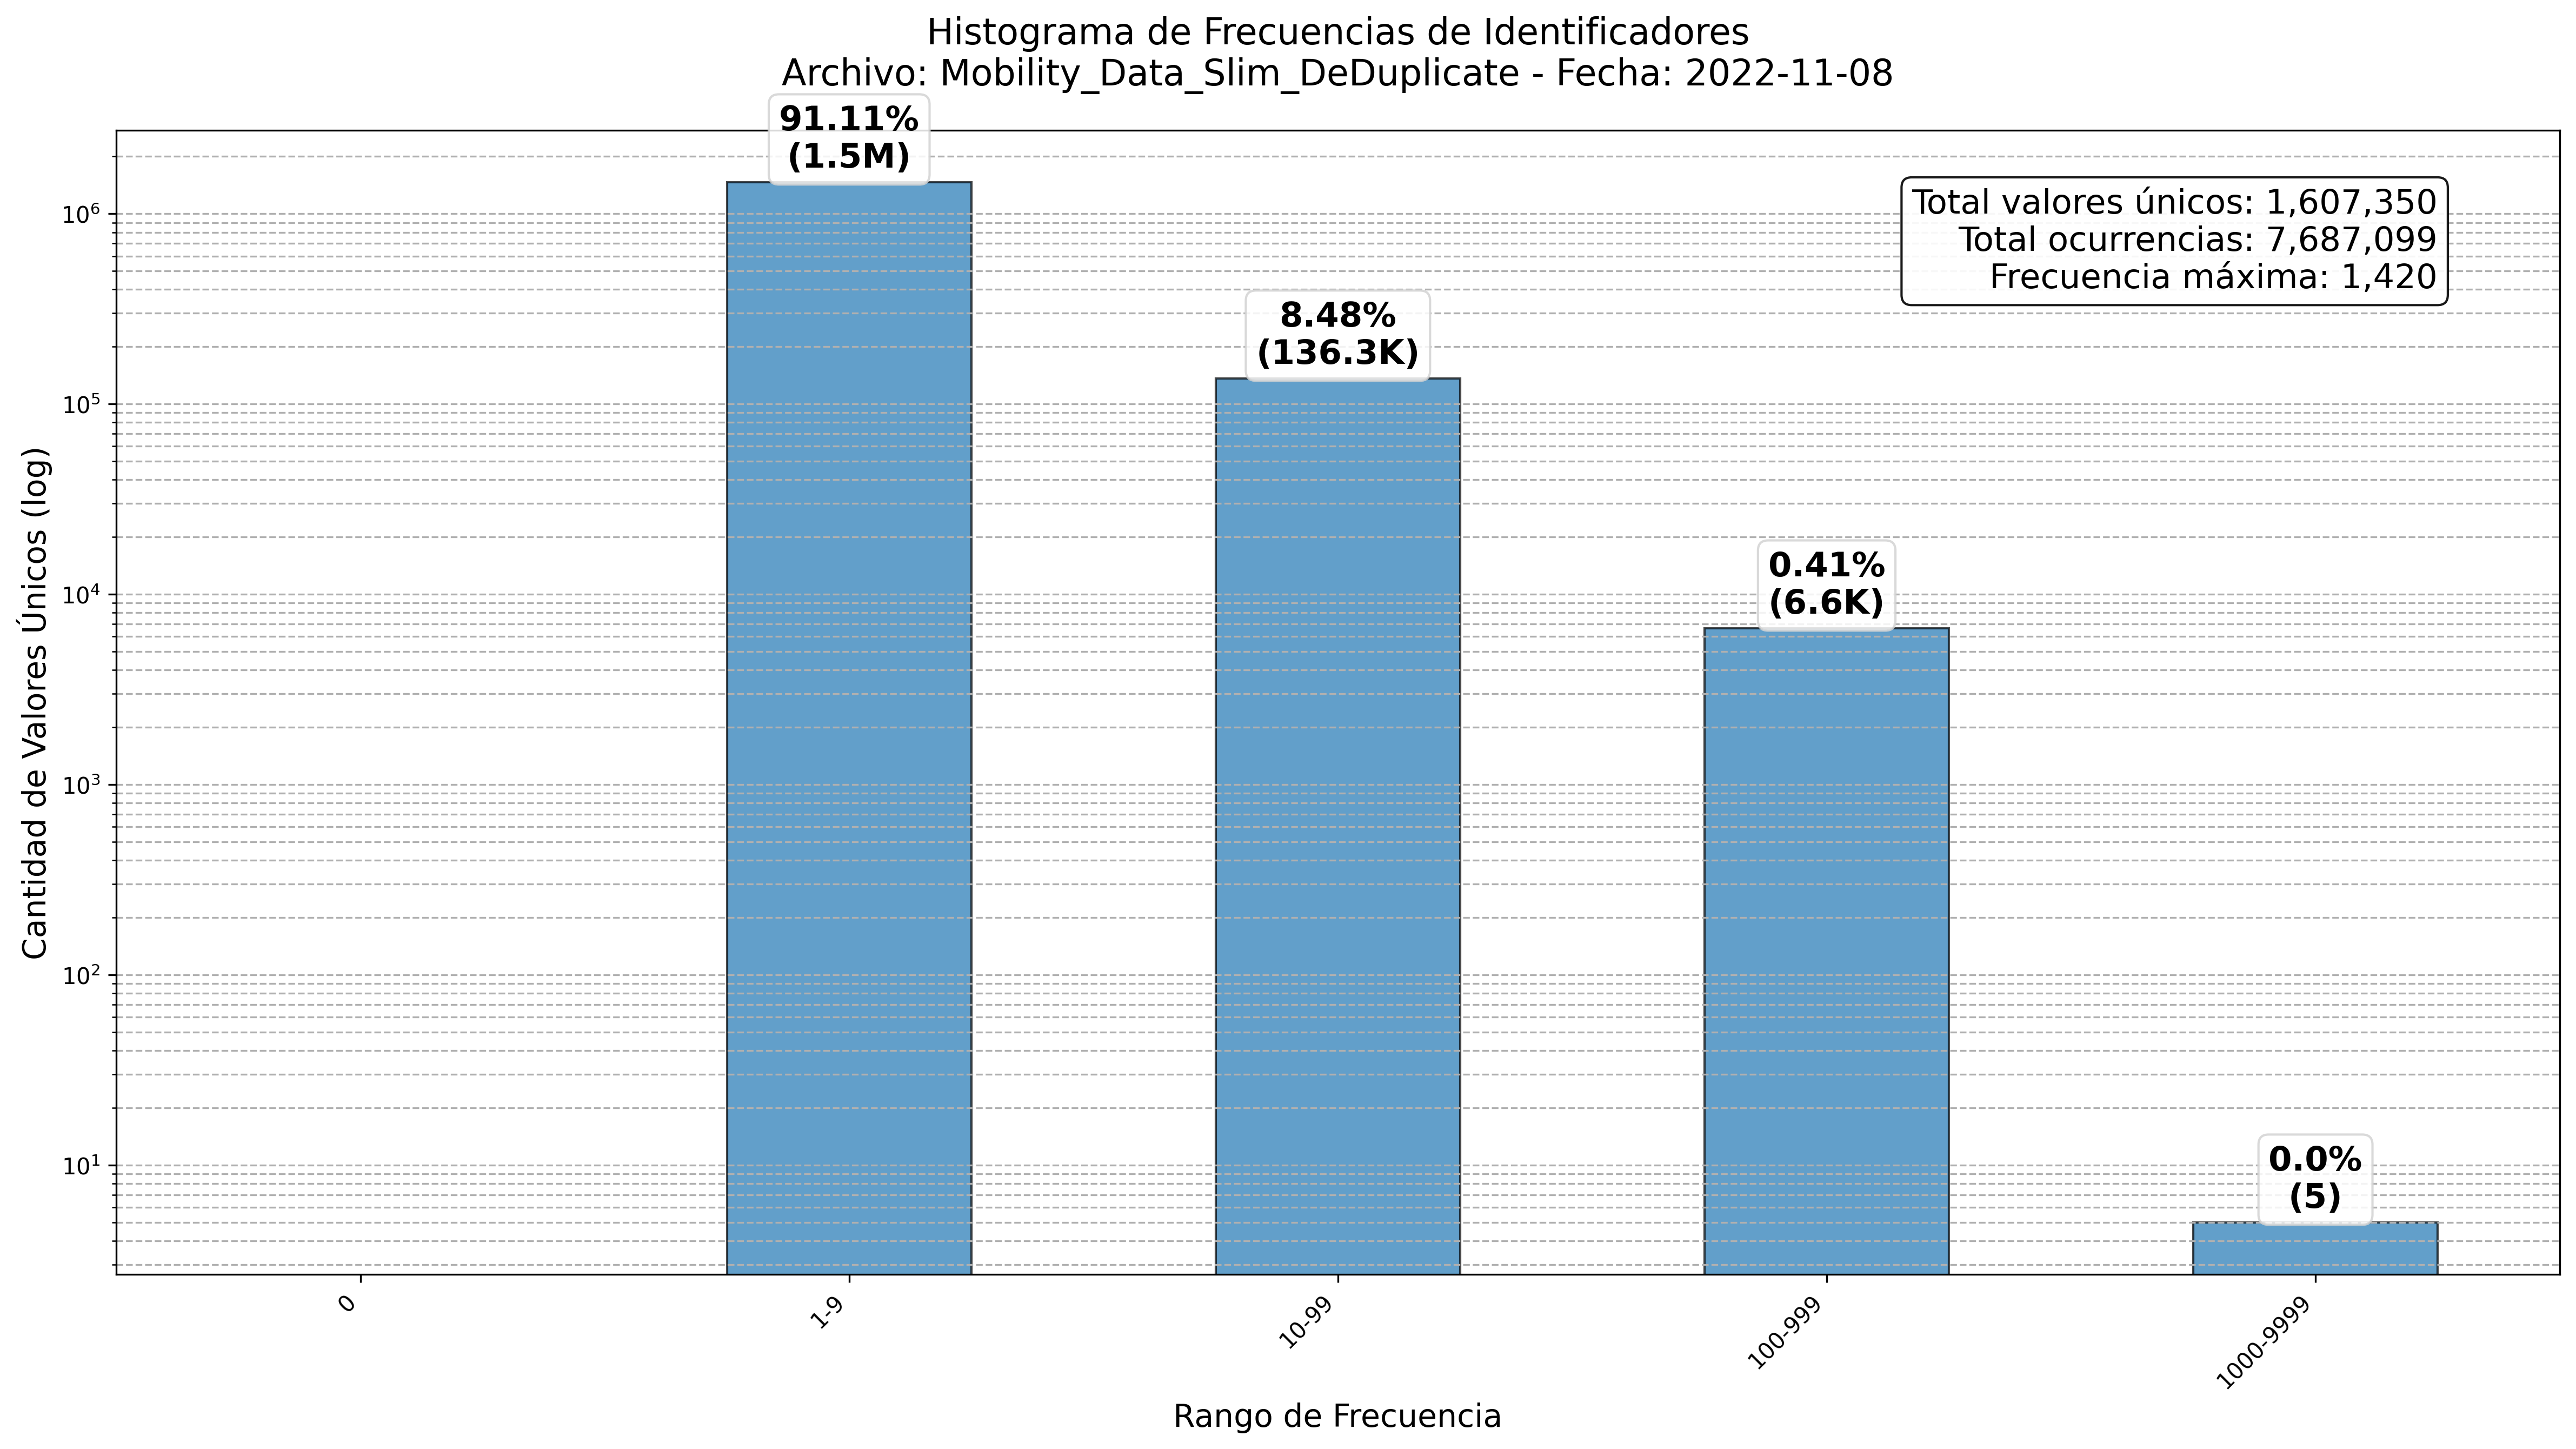
\includegraphics[width=\linewidth]{img/daily_histograms/histograma_identifier_Mobility_Data_Slim_DeDuplicate_2022-11-08.png}
        \caption{Histograma del 08/Nov/2022}
        \label{fig:sub3}
    \end{subfigure}
    \hfill
    \begin{subfigure}[t]{0.48\textwidth-1em}
        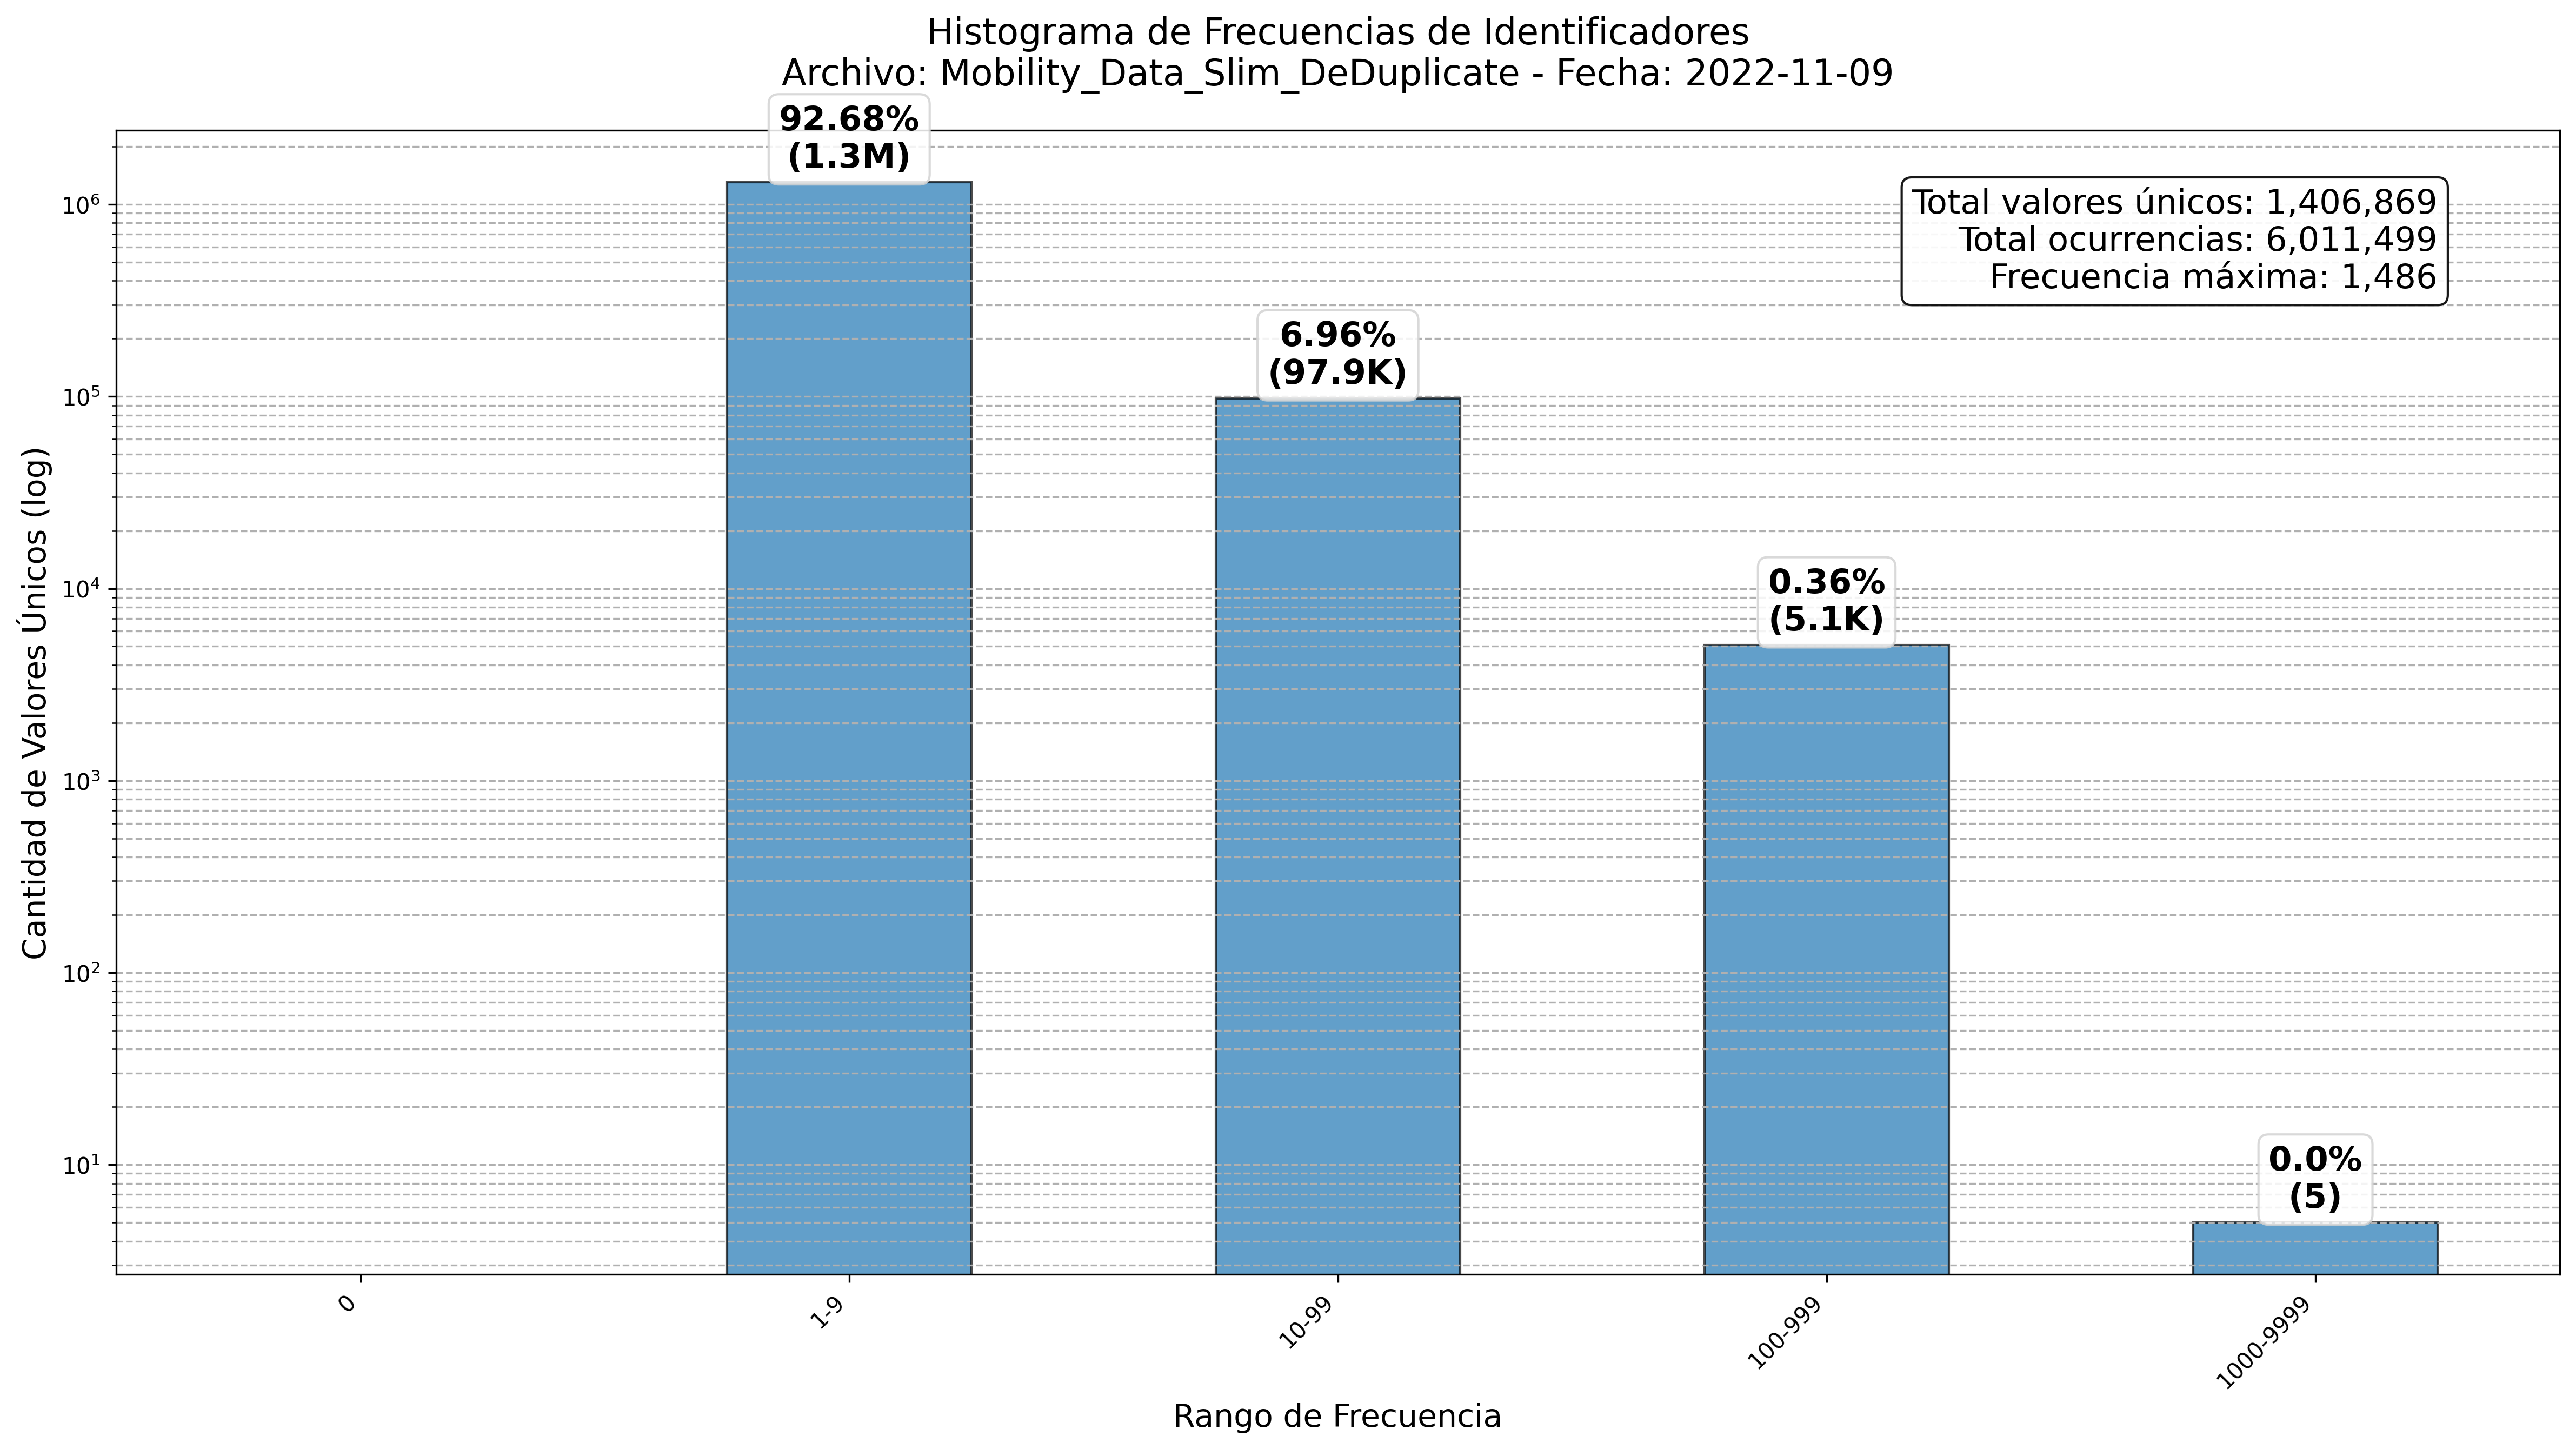
\includegraphics[width=\linewidth]{img/daily_histograms/histograma_identifier_Mobility_Data_Slim_DeDuplicate_2022-11-09.png}
        \caption{Histograma del 09/Nov/2022}
        \label{fig:sub4}
    \end{subfigure}
\end{figure}

\begin{figure}[H]
    \ContinuedFloat
    \centering
    \begin{subfigure}[t]{0.48\textwidth-1em}
        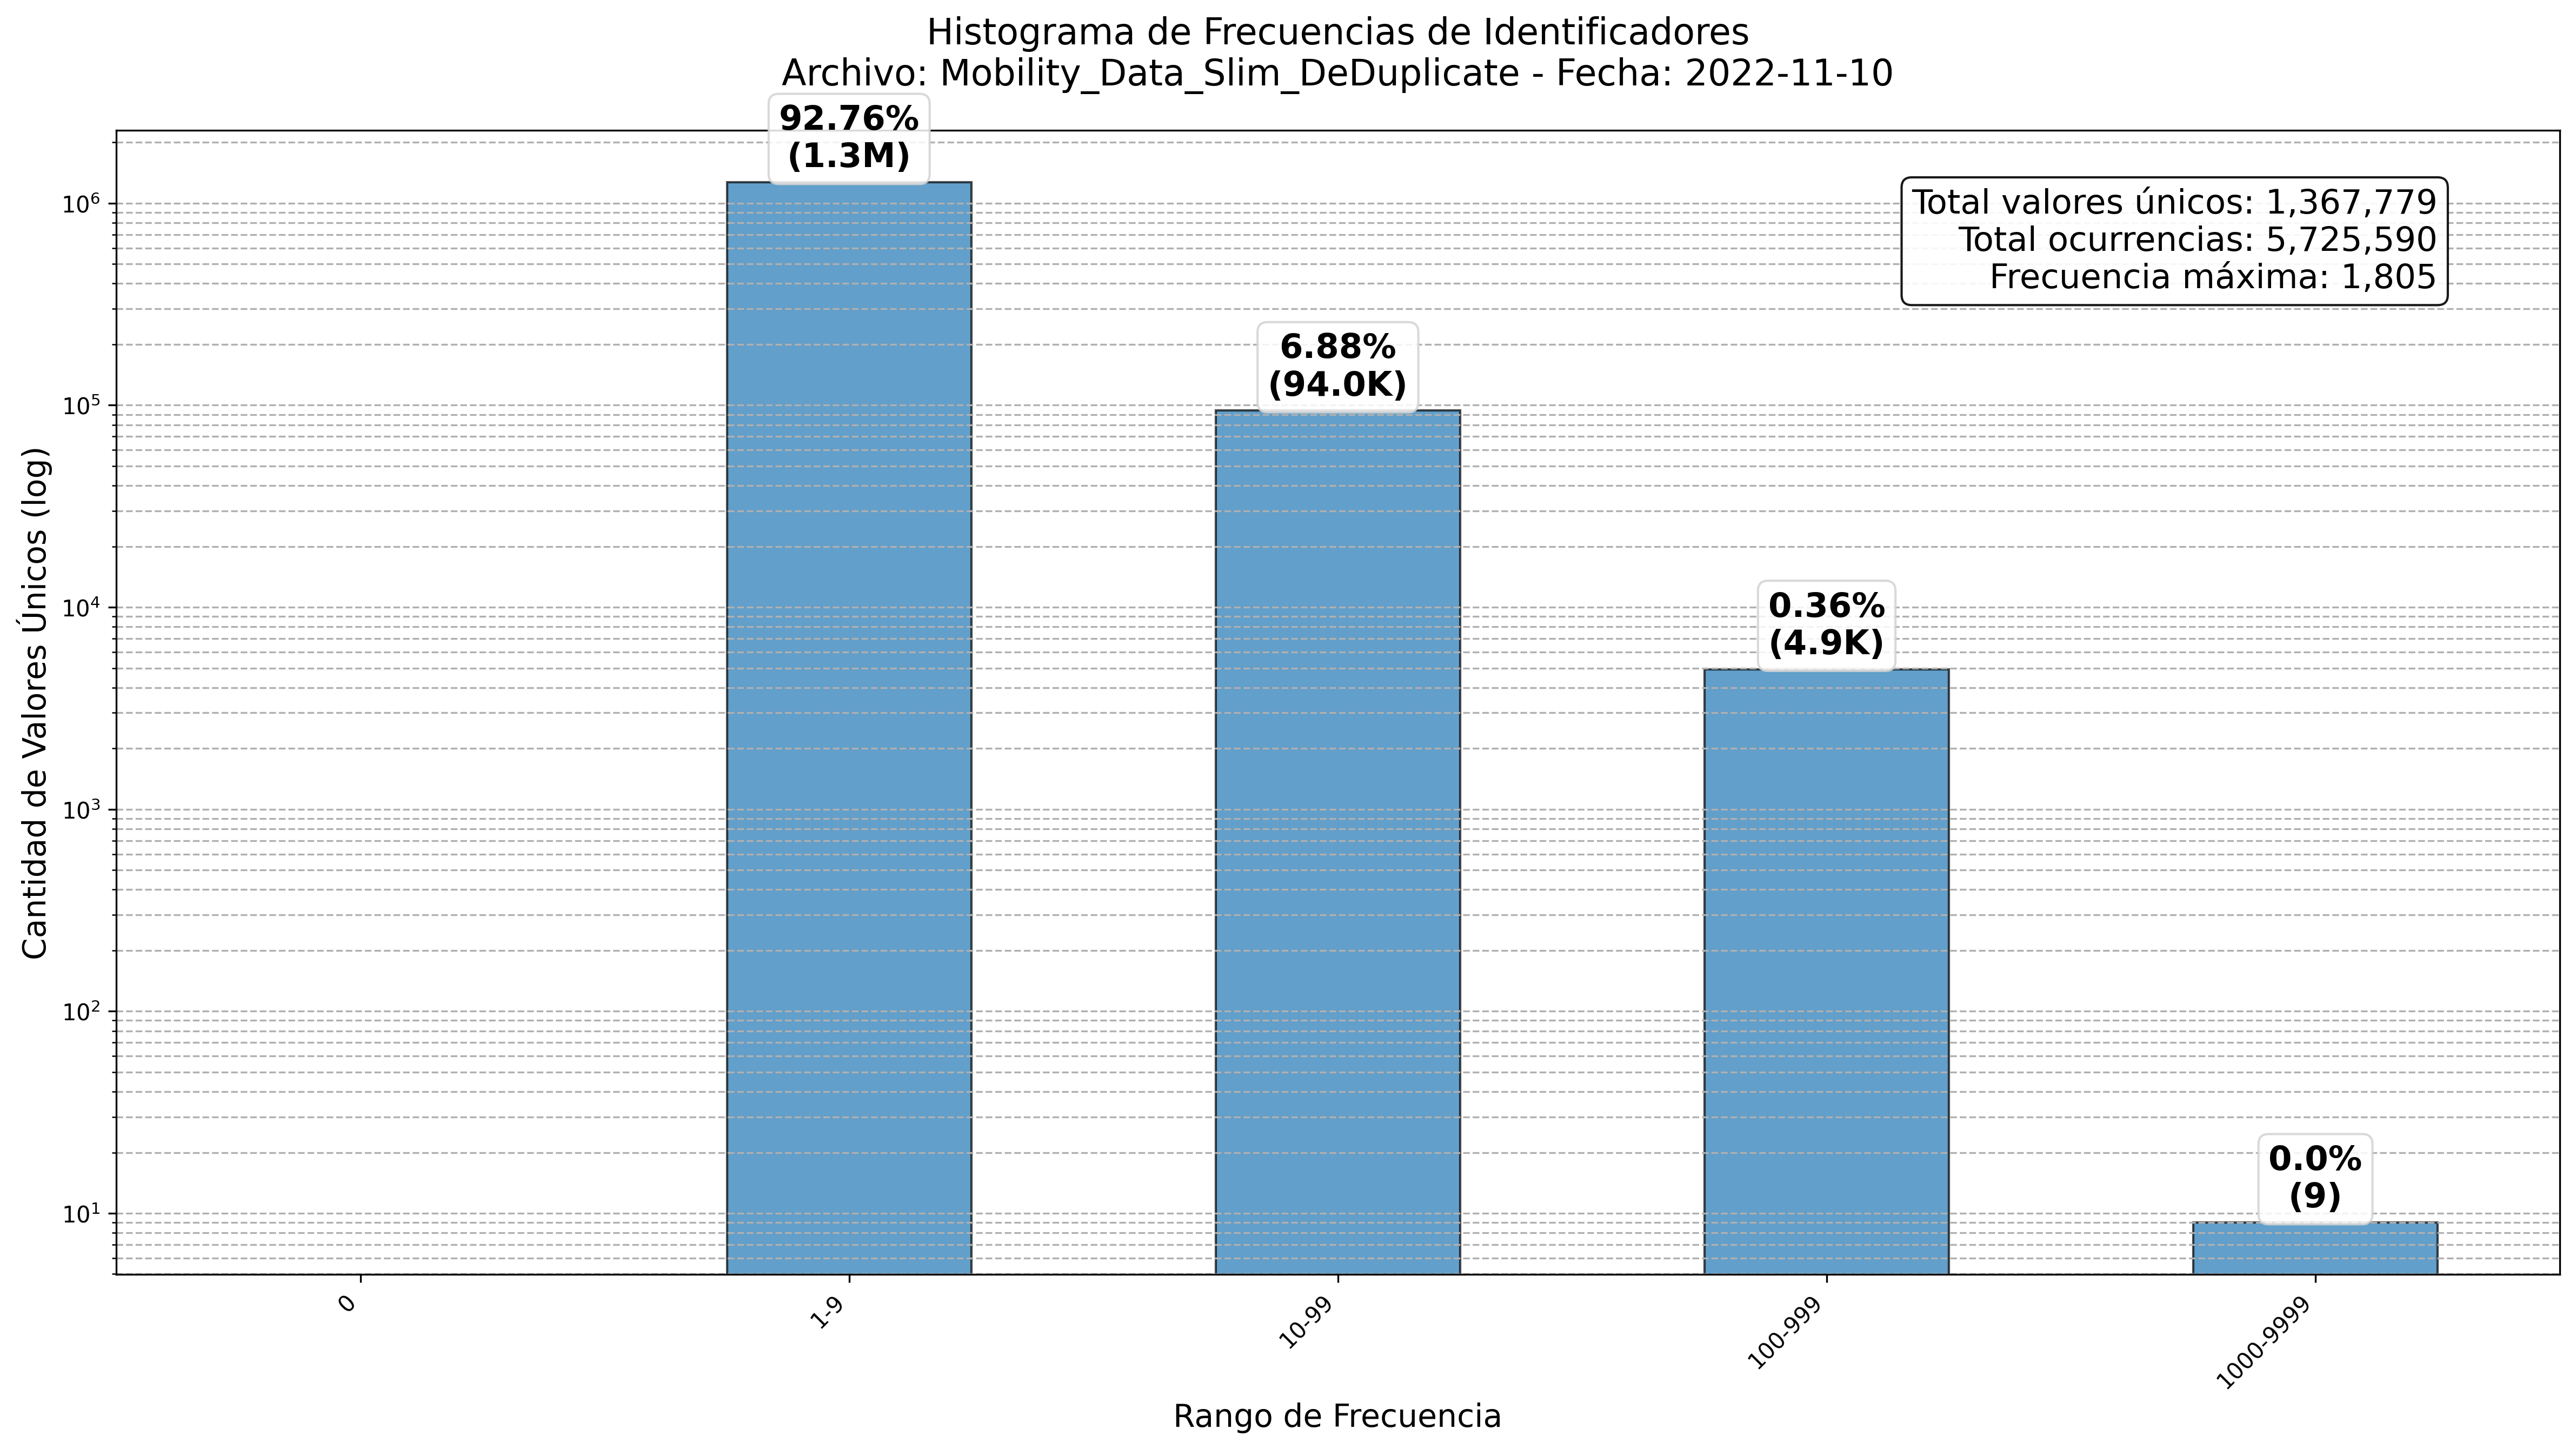
\includegraphics[width=\linewidth]{img/daily_histograms/histograma_identifier_Mobility_Data_Slim_DeDuplicate_2022-11-10.png}
        \caption{Histograma del 10/Nov/2022}
        \label{fig:sub5}
    \end{subfigure}
    \hfill
    \begin{subfigure}[t]{0.48\textwidth-1em}
        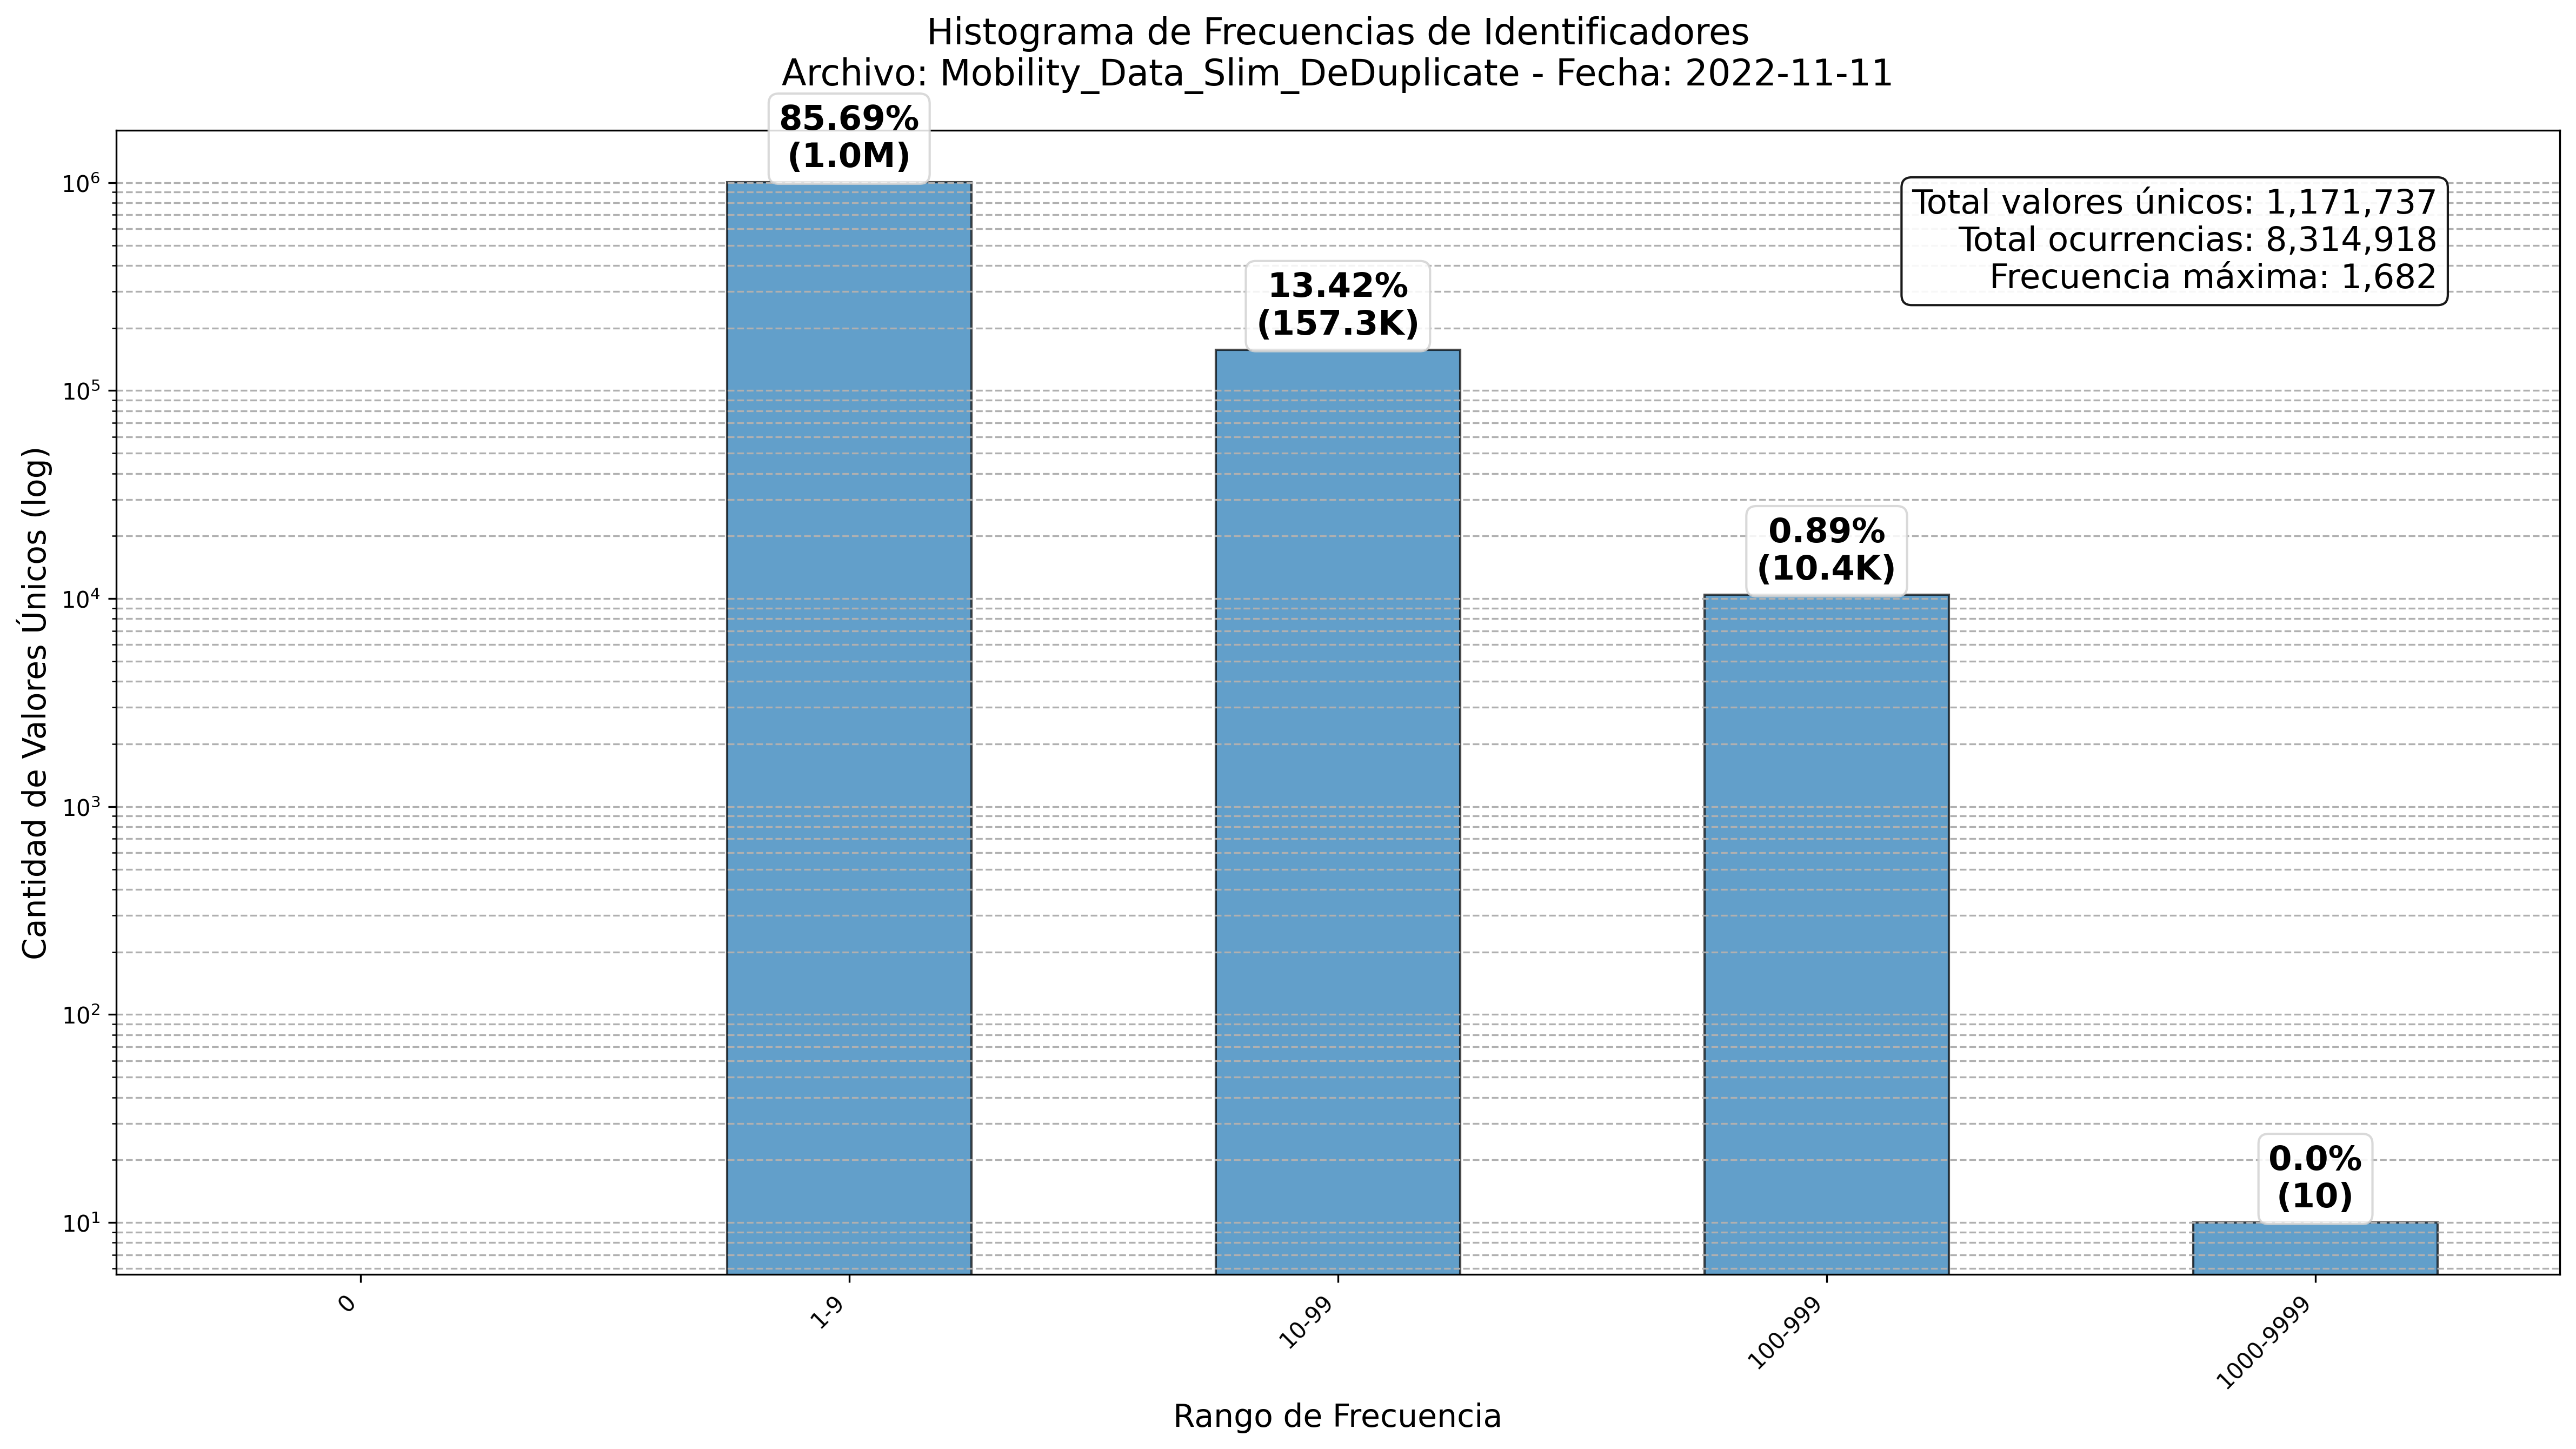
\includegraphics[width=\linewidth]{img/daily_histograms/histograma_identifier_Mobility_Data_Slim_DeDuplicate_2022-11-11.png}
        \caption{Histograma del 11/Nov/2022}
        \label{fig:sub6}
    \end{subfigure}

    \vspace{0.5cm}

    \begin{subfigure}[t]{0.48\textwidth-1em}
        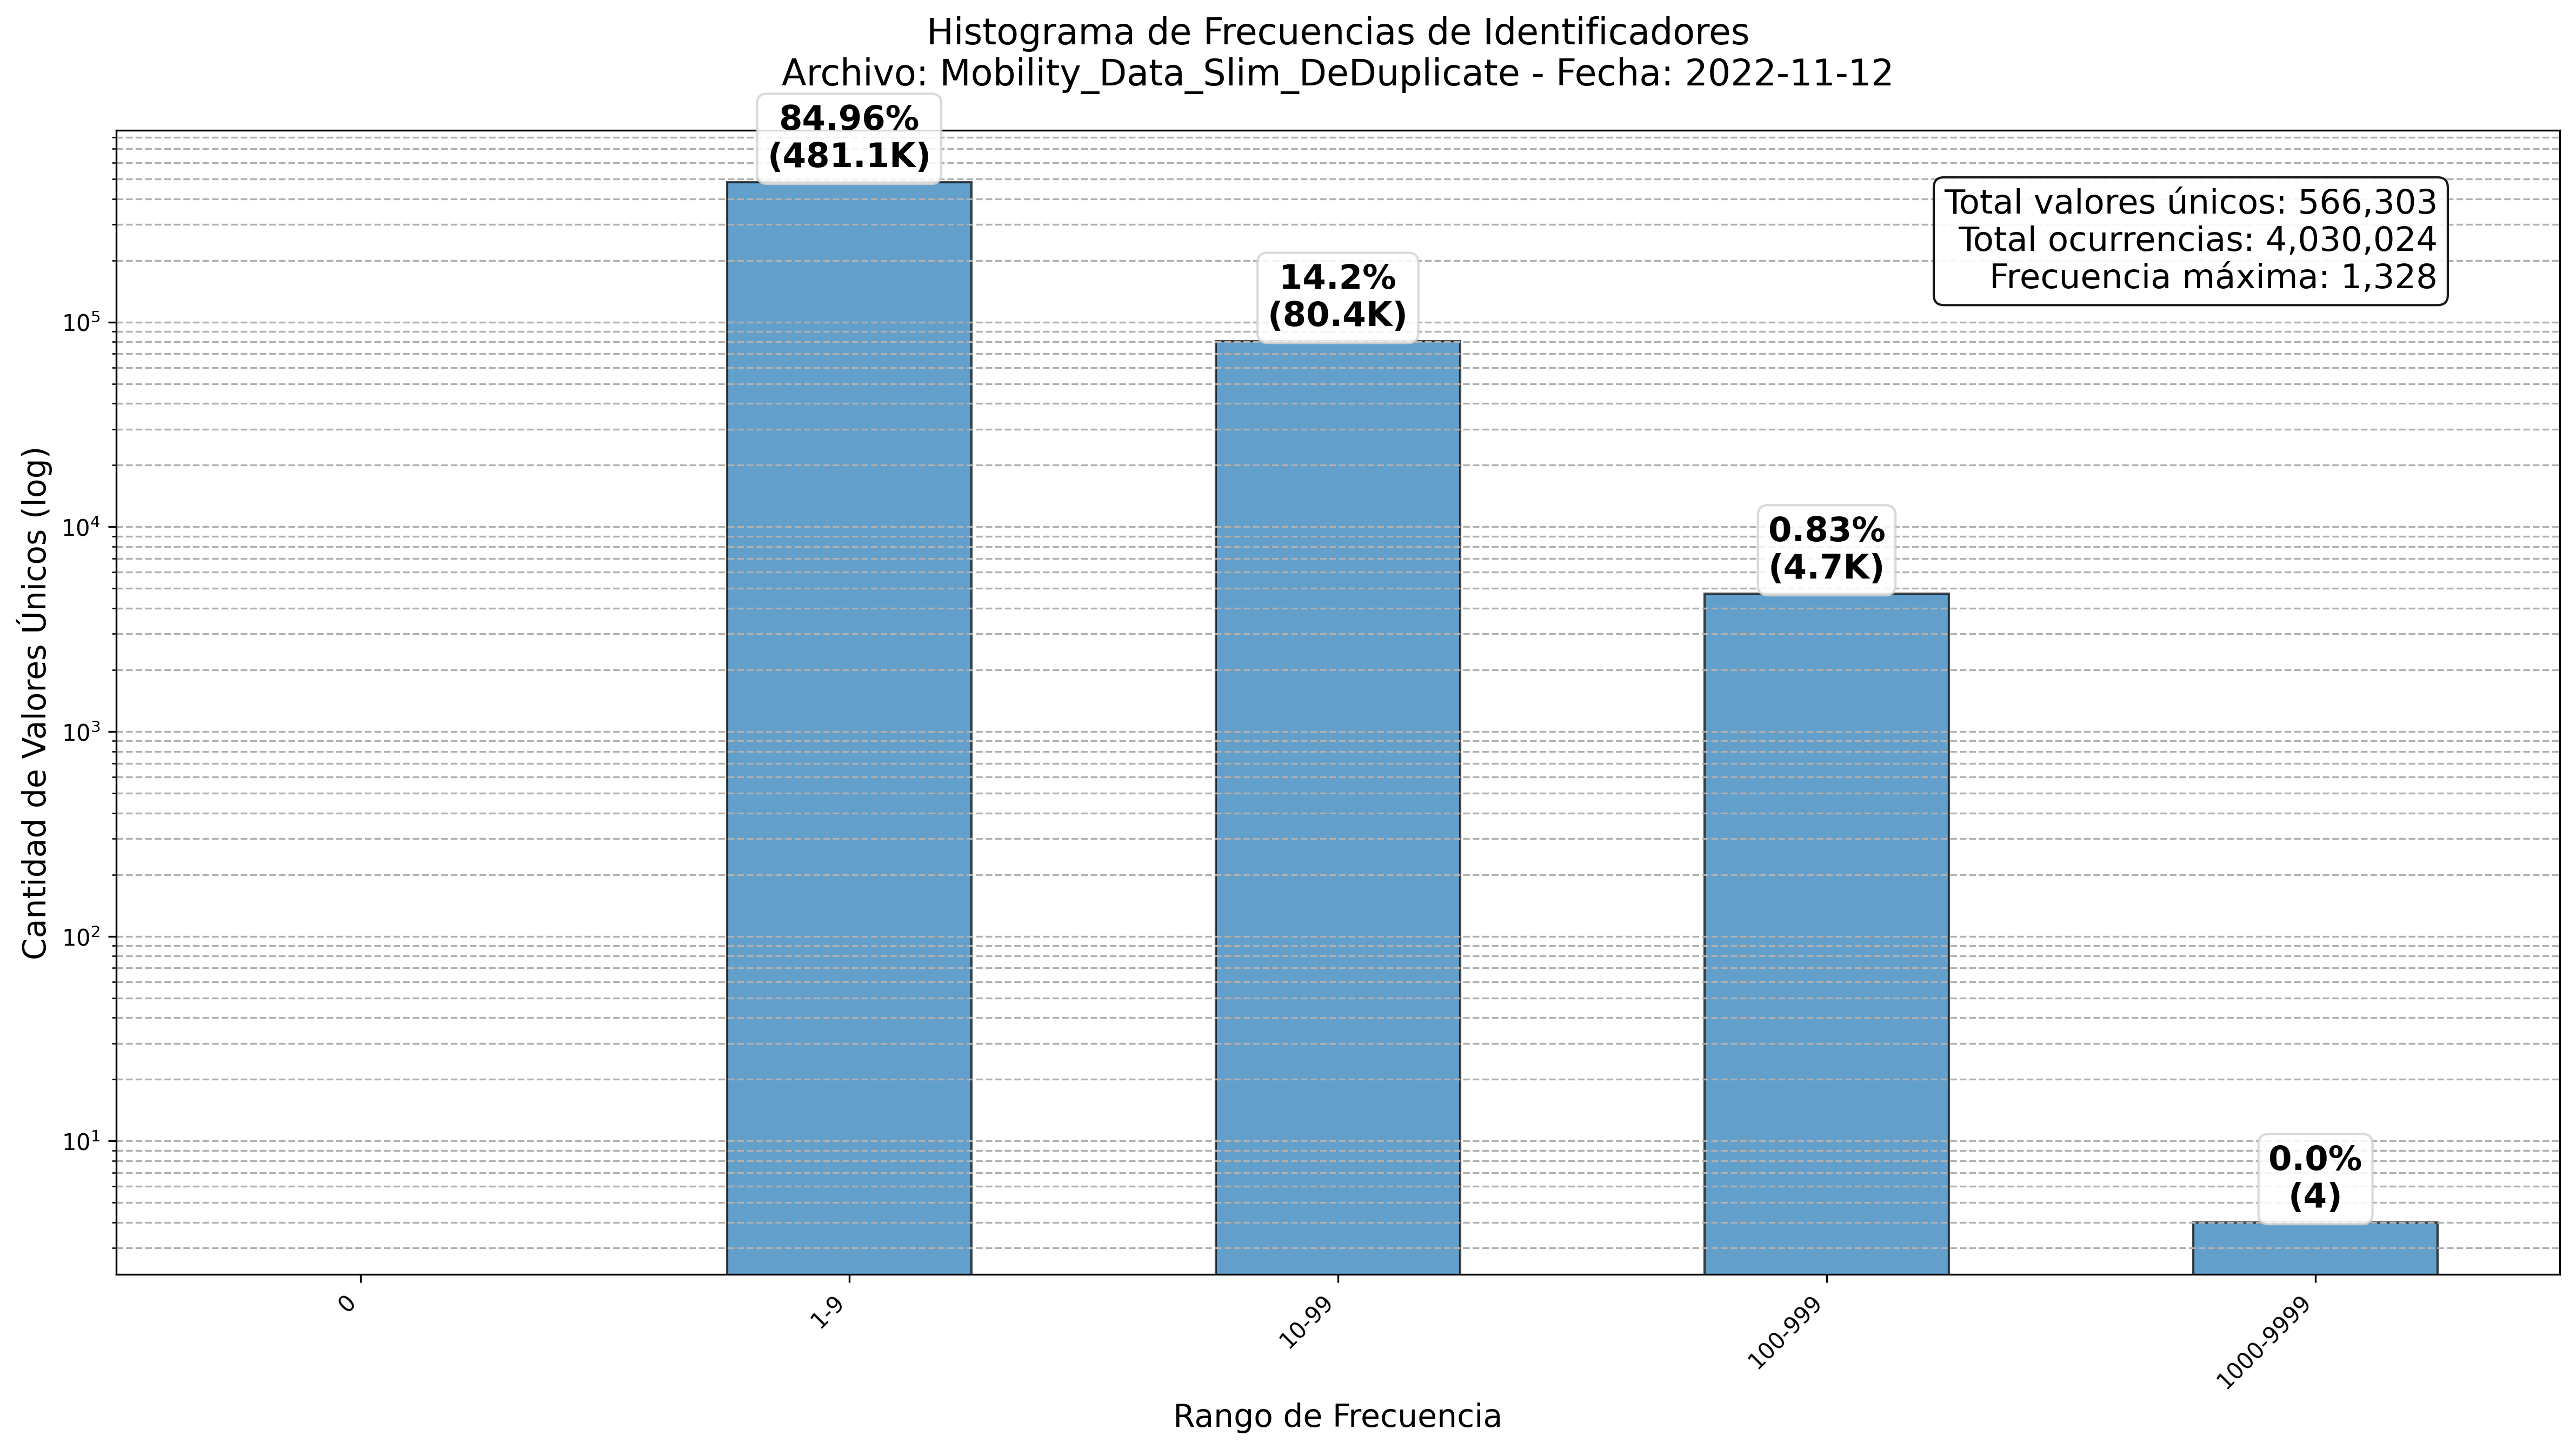
\includegraphics[width=\linewidth]{img/daily_histograms/histograma_identifier_Mobility_Data_Slim_DeDuplicate_2022-11-12.png}
        \caption{Histograma del 12/Nov/2022}
        \label{fig:sub7}
    \end{subfigure}
    \hfill
    \begin{subfigure}[t]{0.48\textwidth-1em}
        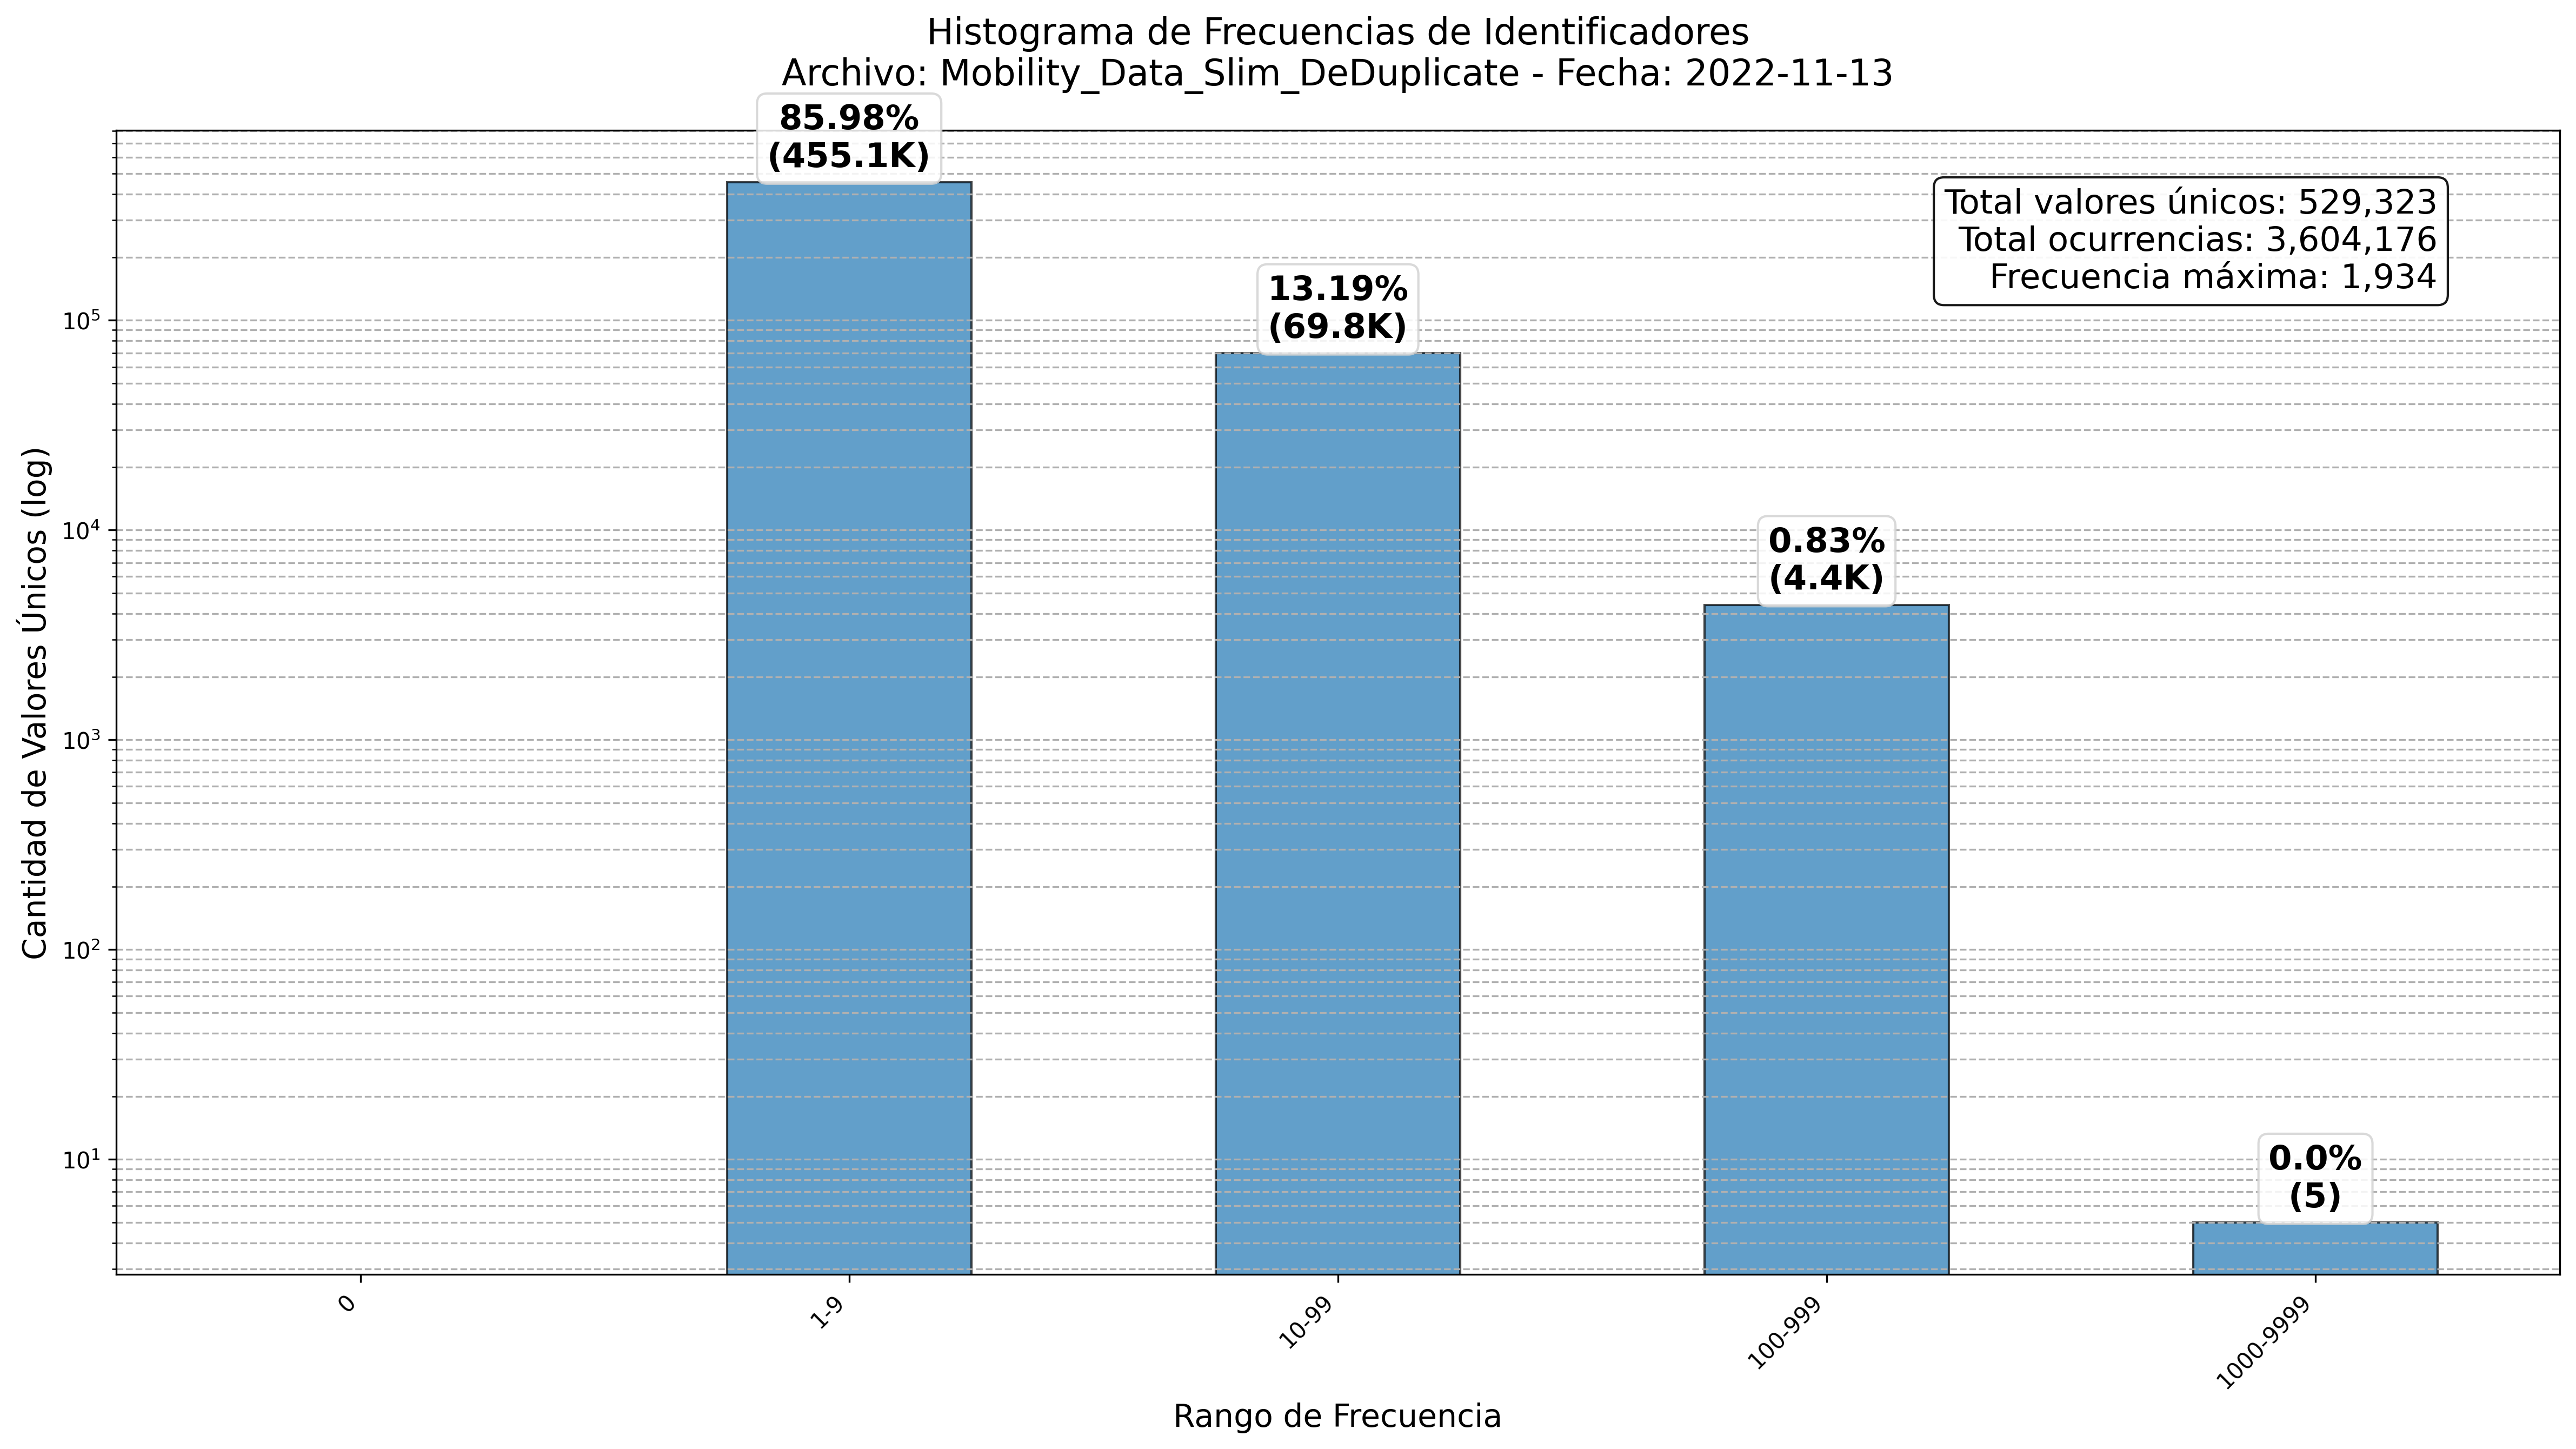
\includegraphics[width=\linewidth]{img/daily_histograms/histograma_identifier_Mobility_Data_Slim_DeDuplicate_2022-11-13.png}
        \caption{Histograma del 13/Nov/2022}
        \label{fig:sub8}
    \end{subfigure}

    \vspace{0.5cm}

    \begin{subfigure}[t]{0.48\textwidth-1em}
        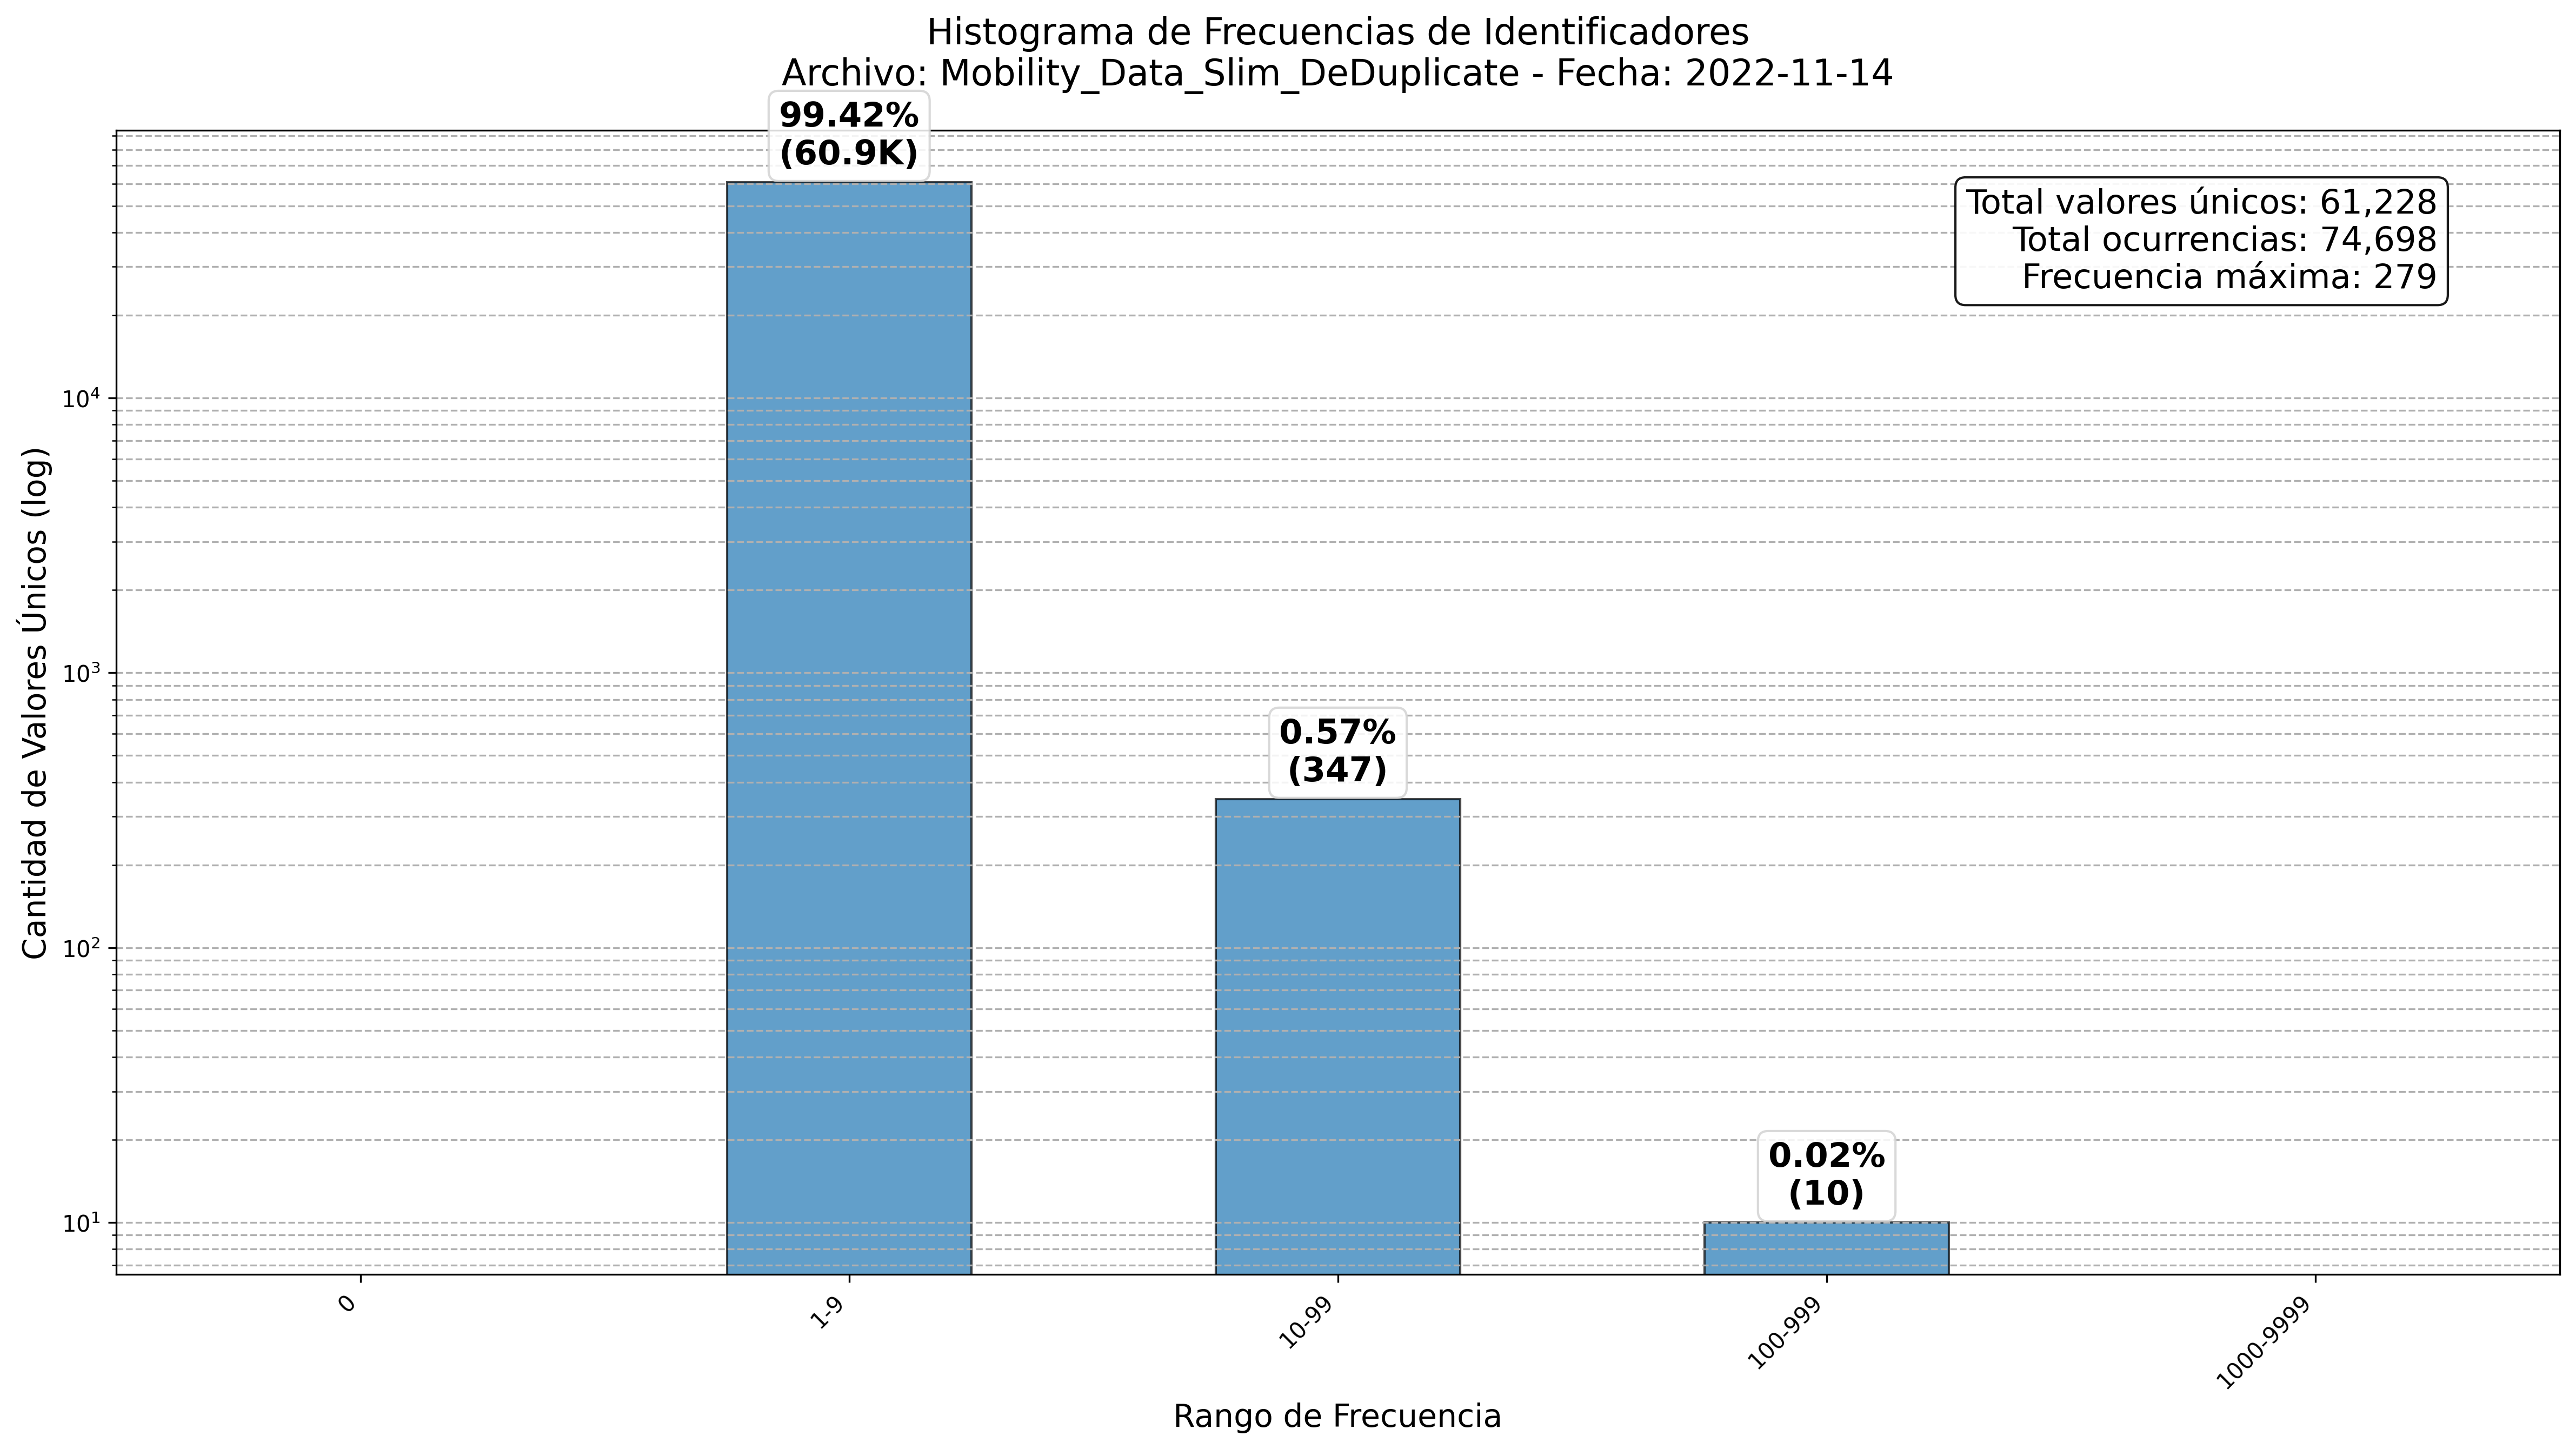
\includegraphics[width=\linewidth]{img/daily_histograms/histograma_identifier_Mobility_Data_Slim_DeDuplicate_2022-11-14.png}
        \caption{Histograma del 14/Nov/2022}
        \label{fig:sub9}
    \end{subfigure}
    \hfill
    \begin{subfigure}[t]{0.48\textwidth-1em}
        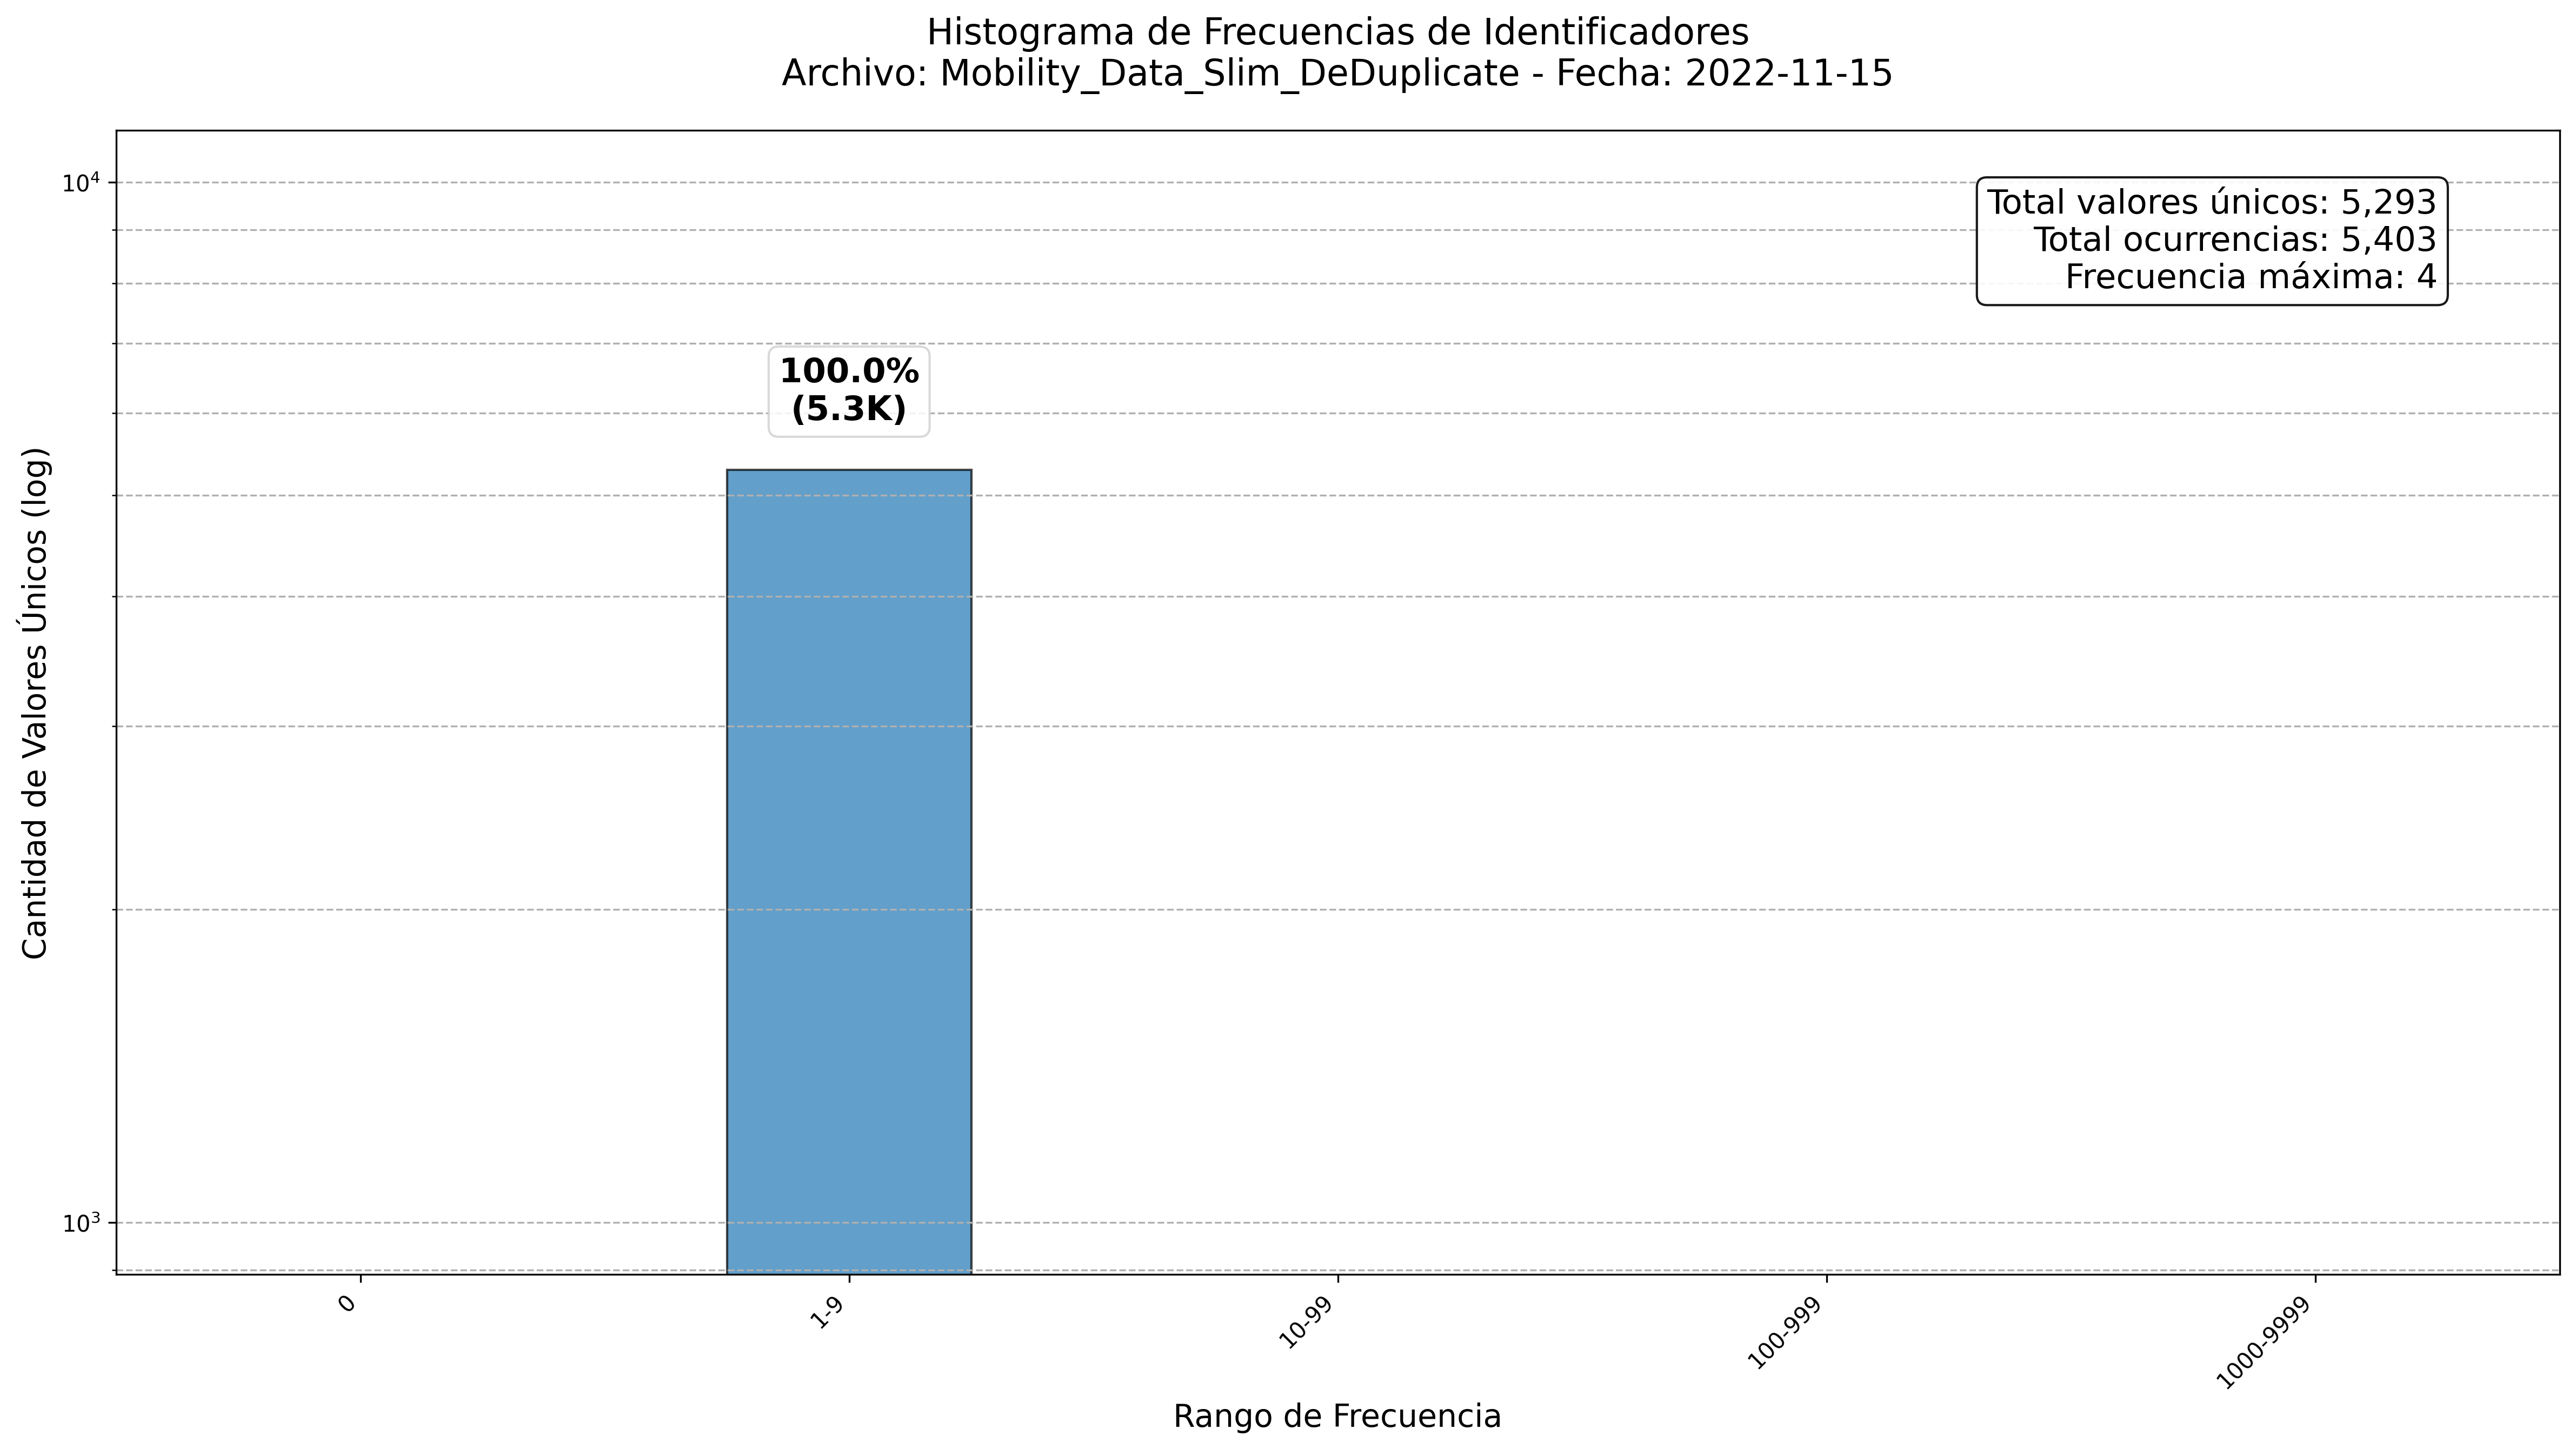
\includegraphics[width=\linewidth]{img/daily_histograms/histograma_identifier_Mobility_Data_Slim_DeDuplicate_2022-11-15.png}
        \caption{Histograma del 15/Nov/2022}
        \label{fig:sub10}
    \end{subfigure}
    \caption{Comparación de distribución de individuos por día.}
    \label{fig:histogramas_daily}
\end{figure}

De la figura anterior se puede observar que la distribución de individuos por día es bastante similar a la distribución vista en la Figura \ref{fig:identifier_histogram_deduplicate}, donde se observa que la mayoría de los individuos tienen una frecuncia de aparición baja. Además se puede ver que los primros seis días hay en promedio \textbf{1,400,000} de individuos, mientras que los últimos cuatro días este valor va disminuyendo hasta llegar a \textbf{5,293} individuos el día 15 de noviembre. Esto puede ser un indicativo de que la recolección de datos no fue constante a lo largo del tiempo, lo que podría deberse a diversos factores como problemas técnicos o cambios en el comportamiento de los individuos.

Un patrón que puede dar mucha información es determinar cuantos individuos tienen puntos de recorrido en más de un día. Para esto se ejecuta el código del Apéndice 

\begin{figure}[H]
  \centering
  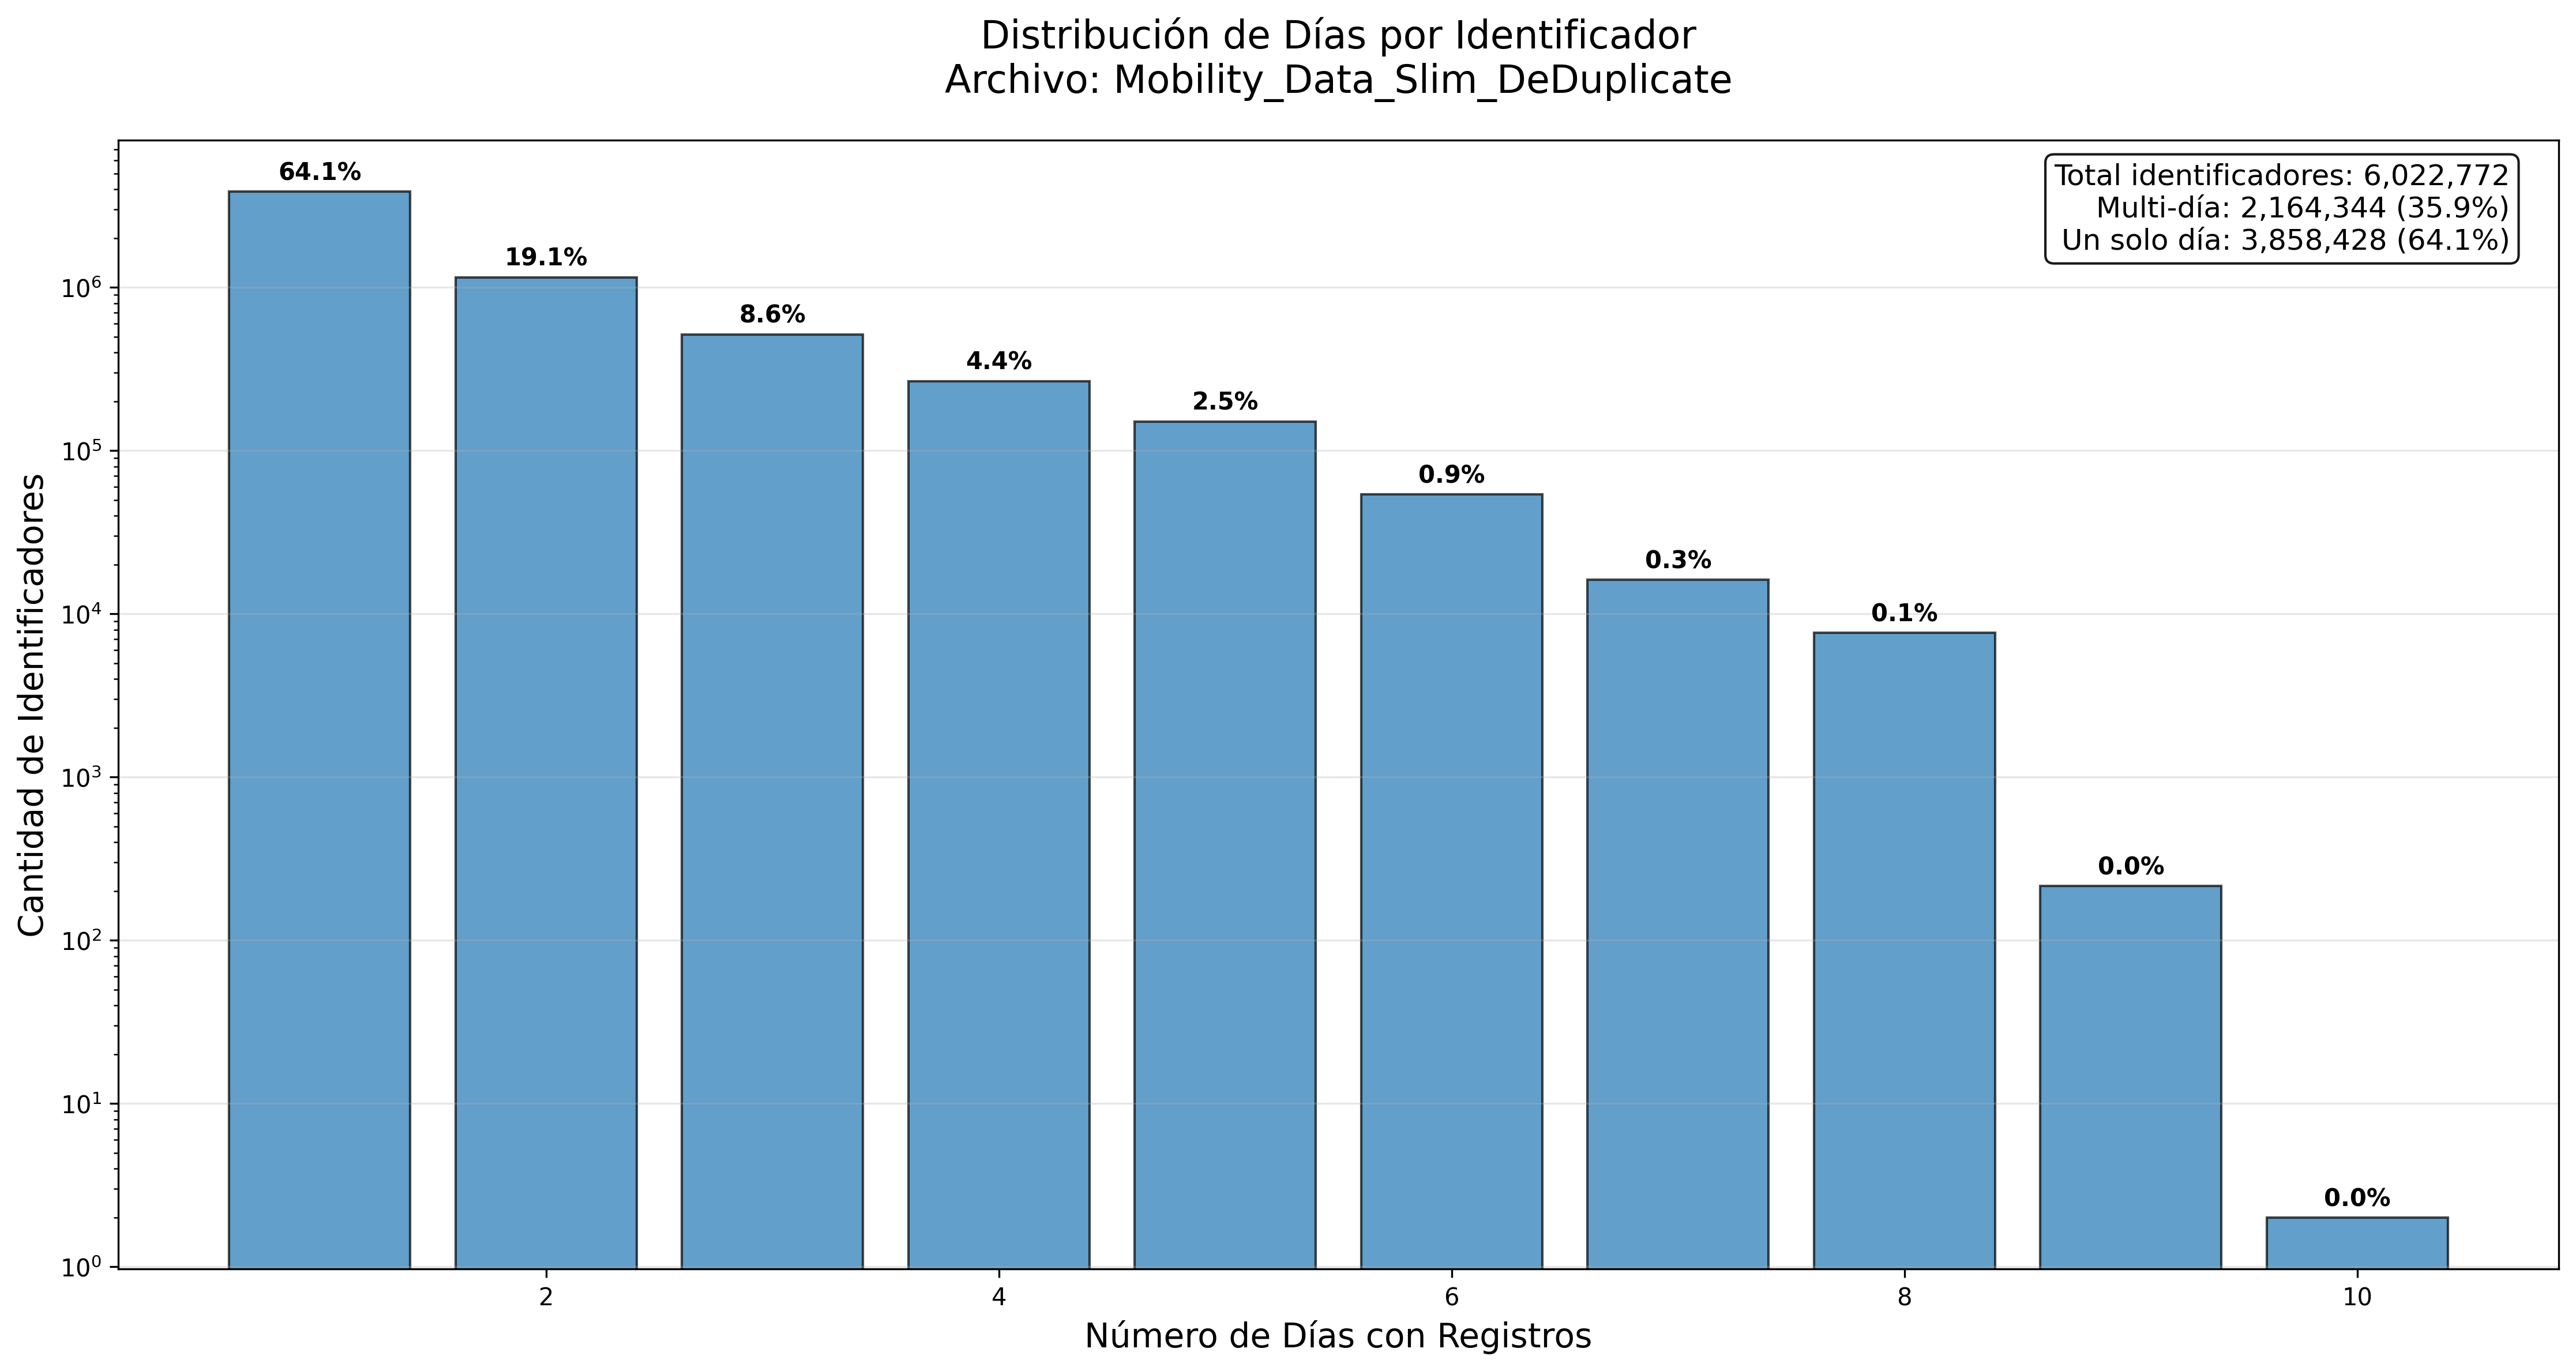
\includegraphics[width=\textwidth]{img/multi_day_analysis_Mobility_Data_Slim_DeDuplicate.png}
  \caption{Distribución de individuos por días.}
  \label{fig:multi_day_analysis}
\end{figure}

El resultado de este análisis se muestra en la figura anterior, donde se puede observar que el \textbf{64.06\%} de los individuos tienen puntos de recorrido en un día nada más, esto representa \textbf{3,858,428} individuos. Por otro lado, el porcentaje de individuos que tienen puntos de recorrido en más de seis días es del \textbf{0.4\%}, lo que representa \textbf{77,878} individuos. Este análisis es importante porque permite identificar a los individuos que tienen un comportamiento más rutinario y que podrían ser más relevantes para el estudio de patrones de movilidad. 

Con esta información se puede realizar un análisis más detallado de las trauectorias de los individuos del conjunto de datos. Por ejemplo, se puede identificar a los individuos que tienen puntos de recorrido en más de un día y que además tienen una alta frecuencia de aparición en esos días. Para esto se puede utilizar un gestor de base de datos como PostgreSQL, que permite realizar consultas complejas y obtener información más detallada sobre los individuos y sus trayectorias.

Para lograr esto, se puede utilizar el servicio de PostgreSQL creado al levantar el contenedor de Docker, como se describe en el Apéndice \ref{cod:docker_compose_file}. Es necesario crear una base de datos y una tabla para almacenar los datos; importar los datos del archivo CSV a esta tabla se hace mediante el código del Apéndice \ref{cod:migrate_csv_to_postgres}. Una vez que los datos están en la base de datos, se pueden realizar consultas para obtener información más detallada sobre los individuos y sus trayectorias. A continuación, se exploraran algunos queries que permiten obtener información relevante sobre los individuos y sus trayectorias.

\newpage
\section{Queries para el análisis de trayectorias individuales}
El primer paso para encontrar las mejores trayectorias es identificar el porcentaje de puntos de recorrido que tienen una precisión de GPS mejor a 20 metros. Para esto se ejecuta el query del Apéndice \ref{cod:query_precision_gps}, cuyo resultado se muestra en la siguiente tabla.

\begin{figure}[H]
    \centering
    \begin{tabular}{@{}cccl@{}} \toprule
        \begin{tabular}[c]{@{}c@{}}
            Total Puntos\\de Recorrido
        \end{tabular} & 
        \begin{tabular}[c]{@{}c@{}}
            Total Puntos de\\Recorrido con\\Precisión GPS
        \end{tabular} &
        \begin{tabular}[c]{@{}c@{}}
            Porcentaje de Puntos de\\Recorrido con\\Precisión GPS
        \end{tabular} & \\ \midrule
        51,077,925 & 34,364,037 & 67.28\% &  \\ \bottomrule 
    \end{tabular}
    \caption{Porcentaje de puntos de recorrido con precisión GPS.}
    \label{fig:precision_gps}
\end{figure}

Debido a que una trayectoria debe tener más un punto de recorrido, para este análisis se consideran únicamente los individuos que tienen más de tres puntos de recorrido. Para así obtener el porcentaje de individuos que cumplen con esta condición. Se ejecuta el query del Apéndice \ref{cod:query_individuos_mas_de_3_registros}, cuyo resultado se muestra en la siguiente tabla.

\begin{figure}[H]
    \centering
    \begin{tabular}{@{}cccl@{}} \toprule
        \begin{tabular}[c]{@{}c@{}}
            Total\\de Individuos
        \end{tabular} & 
        \begin{tabular}[c]{@{}c@{}}
            Individuos con más\\de tres puntos
        \end{tabular} &
        \begin{tabular}[c]{@{}c@{}}
            Porcentaje de Puntos de\\Individuos con\\más de tres puntos
        \end{tabular} & \\ \midrule
        6,022,772 & 2,119,560 & 35.19\% &  \\ \bottomrule 
    \end{tabular}
    \caption{Porcentaje de individuos con más de tres puntos de recorrido.}
    \label{fig:individuos_mas_de_3_puntos}
\end{figure}

Ahora hay que identificar los individuos que tienen más de tres puntos de recorrido y que además tienen una precisión de GPS mejor a 20 metros. Para esto se ejecuta el query del Apéndice \ref{cod:query_individuos_mas_de_3_y_precision}, cuyo resultado se muestra en la siguiente tabla.

\begin{figure}[H]
    \centering
    \begin{tabular}{@{}cccl@{}} \toprule
        \begin{tabular}[c]{@{}c@{}}
            Total\\de Individuos
        \end{tabular} & 
        \begin{tabular}[c]{@{}c@{}}
            Individuos con más\\de tres puntos\\y precisión GPS
        \end{tabular} &
        \begin{tabular}[c]{@{}c@{}}
            Porcentaje de Puntos de\\Individuos con\\más de tres puntos\\ y precisión GPS
        \end{tabular} & \\ \midrule
        6,022,772 & 1,534,172 & 25.47\% &  \\ \bottomrule 
    \end{tabular}
    \caption{Porcentaje de individuos con más de tres puntos de recorrido y precisión GPS.}
    \label{fig:individuos_mas_de_3_y_precision}
\end{figure}

Estos queries permiten identificar la calidad de los datos. A partir de estos se plantea un algoritmo de evaluación de la calidad de las trayectorias, el cual se encuentra en el Apéndice \ref{cod:query_calidad_trayectorias}. El algoritmo inicialmente procesa los datos para identificar movimientos significativos entre registros consecutivos. Se considera movimiento significativo cuando el cambio en coordenadas excede un umbral de 0.001 grados (aproximadamente 111 metros). Para cada individuo se calculan métricas básics de calidad:

\begin{itemize}
    \item \textbf{Volumen de datos (records\_count):} Número total de registros.
    \item \textbf{Cobertura temporal (time\_span\_days):} Duración total en días entre el primer y último registro.
    \item \textbf{Consistencia temporal (active\_days\_count):} Número de días únicos con registros.
    \item \textbf{Calidad técnica (avg\_accuracy\_count):} Precisión promedio del GPS en metros.
    \item \textbf{Riqueza de movimiento (movement\_points):} Número movimientos significativos detectados.
    \item \textbf{Diversidad espacial (spatial\_range):} Rango espacial total cubierto por los registros.
\end{itemize}

Para cada componente se consideran los siguientes criterios de interpretación:

Volumen de Datos (records\_count), un mayor número de registros proporciona más información para el análisis de patrones de movilidad. Trayectorias con >500 registros se consideran ideales, mientras que el mínimo funcional se establece en 50 registros.

Cobertura Temporal (time\_span\_days, active\_days\_count), períodos de observación más extensos permiten capturar patrones de movilidad a largo plazo y variaciones estacionales. El ratio de actividad (activity\_ratio) indica la consistencia de la recolección de datos.

Precisión GPS (avg\_accuracy\_meters), la precisión técnica afecta directamente la confiabilidad de los análisis. Valores <10m se consideran excelentes, 10-30m buenos, y >50m requieren precaución en el análisis.

Riqueza de Movimiento (movement\_points), indica la variabilidad de la trayectoria. Valores altos sugieren patrones de movilidad complejos, mientras que valores bajos indican individuos mayormente estáticos.

Diversidad Espacial (spatial\_diversity), mide el área geográfica cubierta por la trayectoria. Es fundamental para estudios de movilidad urbana que requieren comprensión de patrones espaciales amplios.

El algoritmo permite ajustar diversos parámetros según las características específicas:


Se emplea un sistema de puntuación ponderada que combina estas métricas normalizadas a una escala de 0 a 100. Donde cada componente se calcula como:

\begin{itemize}
    \item \textbf{Volumen (25\%):} min(100, records\_count / 5.0)
    \item \textbf{Duración (20\%):} min(100, time\_span\_days / 0.3)
    \item \textbf{Regularidad (20\%):} min(100, active\_days\_count / time\_span\_days * 100)
    \item \textbf{Precisión (15\%):} max(0, 100 - avg\_accuracy\_meters)
    \item \textbf{Movilidad (10\%):} min(100, movement\_points / 1.0)
    \item \textbf{Diversidad espacial (10\%):} min(100, spatial\_range / 0.01 * 100)
\end{itemize}

El algoritmo genera las siguientes métricas para cada trayectoria evaluada:

\begin{itemize}
    \item \textbf{identifier:} Identificador único del individuo.
    \item \textbf{records\_count:} Volumen total de registros GPS disponibles.
    \item \textbf{time\_span\_days:} Periodo de observación en días.
    \item \textbf{active\_days\_count:} Días únicos con actividad registrada.
    \item \textbf{activity\_ratio:} Proporción de días activos respecto al periodo total (0.0-1.0).
    \item \textbf{avg\_accuracy\_meters:} Precisión promedio del GPS en metros.
    \item \textbf{movement\_points:} Cantidad de desplazamientos significativos detectados.
    \item \textbf{spatial\_range:} Rango geográfico cubierto por la trayectoria.
    \item \textbf{quality\_score:} Puntuación compuesta de calidad (0-100).
    \item \textbf{quality\_category:} Clasificación cualitativa de la trayectoria.
    \item \textbf{overall\_rank:} Posición relativa en el ranking de calidad.
\end{itemize}

Se establecen cinco categorías de calidad basadas en la puntuación compuesta:

\begin{description}
    \item[EXCELENTE:] ($\geq$80)
    \item[MUY BUENA:] ($\geq$65)
    \item[BUENA:] ($\geq$50)
    \item[REGULAR:] ($\geq$35)
    \item[BAJA:] (<35)     
\end{description}


